% !TeX TXS-program:compile = txs:///pdflatex/
% !BIB program = biber



\documentclass[aspectratio=149, 10pt, t]{beamer}

% For the 14:9 aspect ratio, 10pt is a bit small, while 11pt is a bit large
% for my taste. Hence, let’s use 10.5pt:
\renewcommand{\normalsize}{\fontsize{10.5pt}{13pt}\selectfont}
% Bigger sizes like \large, \Large, etc. are identical for the 10pt and 11pt options
% (see http://www.sascha-frank.com/latex-font-size.html), so no need to adjust them.

% !TeX program = pdflatex
% !TeX TXS-program:compile = txs:///pdflatex/
% !TeX TS-program = pdflatex
% !BIB program = biber
% !TeX TXS-program:bibliography = txs:///biber




%%%%%%%%%%%%%%%%%%%%%%%%%%%%
%%  FUNDAMENTAL SETTINGS  %%
%%%%%%%%%%%%%%%%%%%%%%%%%%%%


\newcommand{\serifbodyfont}{0}
% 0: Body is set in sans-serif font
% 1: Body is set in serif font
\newcommand{\serifheadingfont}{0}
% 0: Headings (``structure'') are set in sans-serif font
% 1: Headings (``structure'') are set in serif font

\newcommand{\showsectionnavigation}{0}
% 0: ``Headline'' is disabled.
% 1: ``Headline'' (at the very top of slides) is included and displays all sections of the presentation,
%      with the current section being highlighted.




%%%%%%%%%%%%%%%%%%%%%%%%%%%%
%%  FUNDAMENTAL PACKAGES  %%
%%%%%%%%%%%%%%%%%%%%%%%%%%%%


\usepackage{ifthen}

\usepackage{calc}

\usepackage{tcolorbox}

\usepackage[LY1, LGR, TS1, T1]{fontenc}
% LGR (Greek) is needed to enable the ``sansserif math'' features.
\usepackage[utf8]{inputenc}

\usepackage{tabularx}

\ifxetex
	\usepackage[protrusion=true, expansion=false]{microtype}
\else
	\usepackage[protrusion=true, expansion=false, kerning=true]{microtype}
\fi
% The microtype package enables so-called hanging punctuation. That is, when punctuation like ":", ".", "-", etc. is found at the beginning or end of a line, it is protruded a little into the page margin. This results in "optical margin alignment": the protrusion makes the margin look straighter.


\definecolor{darkgray}{rgb}{0.4,0.4,0.4}

\usepackage[absolute, overlay]{textpos}
\usepackage{graphicx}
\usepackage{amsmath}
%\usepackage{amsfonts}
%\usepackage{amssymb}
\usepackage{epstopdf}
\DeclareGraphicsRule{.tif}{png}{.png}{`convert #1 `dirname #1`/`basename #1 .tif`.png}

\usepackage[ngerman, american, USenglish]{babel}
% German and US English hyphenation and quotation marks
\selectlanguage{USenglish}
\usepackage[autostyle=true]{csquotes}

\usepackage{multirow}

\usepackage{xcolor}
\usepackage{pgf}%,pgfarrows,pgfnodes,pgfshade}
\usepackage{tikz}
\usepackage{pgfplots}
\usetikzlibrary{mindmap, trees, patterns}

\usepackage{xspace}

% \usepackage{eurosym}

%\usepackage{etoolbox}
%	% Enables manipulating LaTeX commmands via \preto, \appto, \patchcmd, etc.
%	% loaded automatically by beamer
\usepackage{xpatch}
% Enables manipulating LaTeX commmands via \xpatchcmd etc.

\hypersetup{%
	pdfpagemode=FullScreen,
	breaklinks=true,
	colorlinks, linkcolor=, urlcolor=SpotColor, citecolor=%
}
\urlstyle{same}
\newcommand{\email}[1]{\href{mailto:#1}{\nolinkurl{#1}}}

\usepackage{import}	 % To allow for relative paths in nested \input's (\import's)




%%%%%%%%%%%%%%%%%%%%%
%%  FONT SETTINGS  %%
%%%%%%%%%%%%%%%%%%%%%


\subimport{0_0_Preamble/}{Preamble_Fonts_Charter_FiraSans}

\ifnum \serifbodyfont=0
	\setbeamerfont{normal text}{family=\sffamily}
	\renewcommand{\familydefault}{\savesffamily}
	\renewcommand{\mddefault}{\savesfmdseries}
	\renewcommand{\bfdefault}{\savesfbfseries}
\else
	\usefonttheme{serif}
	\setbeamerfont{normal text}{family=\rmfamily}
\fi
\ifnum \serifheadingfont=0
	\setbeamerfont{structure}{family=\sffamily, shape=\upshape, series=\bfseries}
\else
	\setbeamerfont{structure}{family=\rmfamily, shape=\upshape, series=\bfseries}
\fi

% Make frame titles and headings bold
\usefonttheme{structurebold}
\usefonttheme{professionalfonts}

\setbeamerfont{footline}
	{parent=structure, size=\tiny, series=\mdseries}
\setbeamercolor{footline}
	{fg=SpotColor}

%% Use the bm (= boldmath) package for better support of setting math in bold ==>
%% Prevent the "Too many math fonts used" error:
\newcommand{\bmmax}{0}
\newcommand{\hmmax}{0}
\usepackage{bm}
%% <==

\usepackage{fontawesome}

\usepackage{mathtools}
%\mathtoolsset{centercolon}
% This makes the compilation fail in combination with tikz. See
% https://tex.stackexchange.com/questions/89467/why-does-pdftex-hang-on-this-file.
%% Inspired by https://tex.stackexchange.com/questions/251460/how-to-put-symbols-of-equal-size-on-top-of-each-other
\newcommand{\succeqq}{%
	\mathrel{%
		\vcenter{\offinterlineskip
			\ialign{##\cr$\succ$\cr\noalign{\kern 1pt}$=$\cr}%
		}%
	}%
}
\newcommand{\nsucceqq}{\mathrel{\not\succeqq}}
\newcommand*{\coloneqq}{\mathrel{%
		\mathrel{%
			\raisebox{0.15ex}{\scalebox{0.85}{\ensuremath{:}}}\hspace{-0.2pt}%
		}%
		=%
}}

% !TeX program = pdflatex
% !TeX TXS-program:compile = txs:///pdflatex/
% !TeX TS-program = pdflatex
% !BIB program = biber
% !TeX TXS-program:bibliography = txs:///biber




%%%%%%%%%%%%%%%%%%%%%%%%%%%%%%%%%%%%%%%%%%%%%%%%%
%%  SANS-SERIF MATH IN SANS-SERIF ENVIRONMENT  %%
%%%%%%%%%%%%%%%%%%%%%%%%%%%%%%%%%%%%%%%%%%%%%%%%%


% See https://tex.stackexchange.com/questions/41497/how-to-typeset-some-text-including-math-content-in-sans-serif
% See https://tex.stackexchange.com/questions/33165/make-mathfont-respect-the-surrounding-family

% Necessary for use of kpfonts
% ==>
\makeatletter
\newif\ifkp@upRm
\newif\ifkp@osm
\newif\ifkp@vosm
\makeatother
% <==

\DeclareMathVersion{normalup}
\DeclareMathVersion{boldup}
\DeclareMathVersion{sans}

%\SetSymbolFont{operators}{sans}{OT1}{jkpss}{m}{n}
%	% From http://mirrors.ctan.org/fonts/kpfonts/latex/kpfonts.sty
\SetSymbolFont{operators}   {sans}{OT1}{mdbch}{m}{n}
\SetSymbolFont{letters}     {sans}{OML}{jkpss}{m}{it}
	% From http://mirrors.ctan.org/fonts/kpfonts/latex/kpfonts.sty
%\SetSymbolFont{letters}     {sans}{OML}{cmbrm}{m}{it}
%\SetSymbolFont{symbols}     {sans}{OMS}{cmbrs}{m}{n}
\SetSymbolFont{symbols}     {sans}{OMS}{jkp}  {m}{n}
	% From http://mirrors.ctan.org/fonts/kpfonts/latex/kpfonts.sty
\DeclareSymbolFont{extrasymbols}  {OMS}{cmbrs}{m}{n}
\SetSymbolFont{extrasymbols}{sans}{OMS}{cmbrs}{m}{n}
	% Some symbols (e.g., \prime) look weird in kpfonts.
	% This provides the option to replace them by symbols from mathdesign-charter.

\SetMathAlphabet{\mathit} {sans}{T1}{\savesffamily}{\savesfmdseries}{it}
\SetMathAlphabet{\mathbf} {sans}{T1}{\savesffamily}{\savesfbfseries}{n}
\SetMathAlphabet{\mathtt} {sans}{OT1}{cmtl}{m}{n}
\SetMathAlphabet{\mathcal}{sans}{OMS}{ntxsy}{m}{n}
	% See https://tex.stackexchange.com/questions/231583/import-mathcal-symbols-from-txfonts
%\SetSymbolFont{largesymbols}{sans}{OMX}{jkpss}{m}{n}
%	% From http://mirrors.ctan.org/fonts/kpfonts/latex/kpfonts.sty
\SetSymbolFont{largesymbols} {sans}{OMX}{mdbch}{m}{n}
	% Using symbols like \int, \left(, etc. from mathdesign-charter because they look better than the ones included in kpfonts

\DeclareMathVersion{sansup}
\SetSymbolFont{letters}  {sansup}{OML}{jkpss}{m}{it}
\SetSymbolFont{symbols}  {sansup}{OMS}{jkp}  {m}{n}

\DeclareMathVersion{boldsans}
%\SetSymbolFont{operators}{boldsans}{OT1}{jkpss}{b}{n}
%	% From http://mirrors.ctan.org/fonts/kpfonts/latex/kpfonts.sty
\SetSymbolFont{operators}{boldsans}{OT1}{mdbch}{bx}{n}
\SetSymbolFont{letters}  {boldsans}{OML}{jkpss}{bx}{it}
	% From http://mirrors.ctan.org/fonts/kpfonts/latex/kpfonts.sty
%\SetSymbolFont{letters}  {boldsans}{OML}{mdbch}{bx}{it}
%\SetSymbolFont{letters}{boldsans}{OML}{cmbrm}{b}{it}
\SetSymbolFont{symbols}  {boldsans}{OMS}{jkp}  {bx}{n}
	% From http://mirrors.ctan.org/fonts/kpfonts/latex/kpfonts.sty
%\SetMathAlphabet{\mathrm}{boldsans}{OT1}{\savesffamily}{\savesfbfseries}{n}
\SetMathAlphabet{\mathit} {boldsans}{T1}{\savesffamily}{\savesfbfseries}{it}
\SetMathAlphabet{\mathtt} {boldsans}{T1}{cmtl}{b}{n}
\SetMathAlphabet{\mathcal}{boldsans}{OMS}{ntxsy}{b}{n}
%\SetSymbolFont{largesymbols}{boldsans}{OMX}{jkpss}{bx}{n}
%	% From http://mirrors.ctan.org/fonts/kpfonts/latex/kpfonts.sty
\SetSymbolFont{largesymbols}{boldsans}{OMX}{mdbch}{bx}{n}
	% Using symbols like \int, \left(, etc. from mathdesign-charter because they look better than the ones included in kpfonts

\DeclareMathVersion{boldsansup}
\SetSymbolFont{letters}{boldsansup}{OML}{jkpss}{bx}{it}
\SetSymbolFont{symbols}{boldsansup}{OMS}{jkp}  {bx}{n}

% Adapted from mdbch.sty
\SetSymbolFont{operators}     {boldup}{OT1}{mdbch}{b}{n}%
\SetSymbolFont{letters}       {boldup}{OML}{mdbch}{b}{n}%{it}%
\SetSymbolFont{lettersupright}{boldup}{OML}{mdbch}{b}{n}%
\SetSymbolFont{symbols}       {boldup}{OMS}{mdbch}{b}{n}%
\SetSymbolFont{largesymbols}  {boldup}{OMX}{mdbch}{b}{n}%

% Using glyphs for math mode from the custom sansserif font
\DeclareSymbolFont{uprightglyphs}{T1}{\savermfamily}{\savermmdseries}{n}
\SetSymbolFont{uprightglyphs}{normal}    {T1}{\savermfamily}{\savermmdseries}{n}
\SetSymbolFont{uprightglyphs}{normalup}  {T1}{\savermfamily}{\savermmdseries}{n}
\SetSymbolFont{uprightglyphs}{bold}      {T1}{\savermfamily}{\savermbfseries}{n}
\SetSymbolFont{uprightglyphs}{boldup}    {T1}{\savermfamily}{\savermbfseries}{n}
\SetSymbolFont{uprightglyphs}{sans}      {T1}{\savesffamily}{\savesfmdseries}{n}
\SetSymbolFont{uprightglyphs}{sansup}    {T1}{\savesffamily}{\savesfmdseries}{n}
\SetSymbolFont{uprightglyphs}{boldsans}  {T1}{\savesffamily}{\savesfbfseries}{n}
\SetSymbolFont{uprightglyphs}{boldsansup}{T1}{\savesffamily}{\savesfbfseries}{n}
\DeclareSymbolFont{italicglyphs} {T1}{\savermfamily}{\savermmdseries}{it}
\SetSymbolFont{italicglyphs} {normal}    {T1}{\savermfamily}{\savermmdseries}{it}
\SetSymbolFont{italicglyphs} {normalup}  {T1}{\savermfamily}{\savermmdseries}{n}
\SetSymbolFont{italicglyphs} {bold}      {T1}{\savermfamily}{\savermbfseries}{it}
\SetSymbolFont{italicglyphs} {boldup}    {T1}{\savermfamily}{\savermbfseries}{n}
\SetSymbolFont{italicglyphs} {sans}      {T1}{\savesffamily}{\savesfmdseries}{it}
\SetSymbolFont{italicglyphs} {sansup}    {T1}{\savesffamily}{\savesfmdseries}{n}
\SetSymbolFont{italicglyphs} {boldsans}  {T1}{\savesffamily}{\savesfbfseries}{it}
\SetSymbolFont{italicglyphs} {boldsansup}{T1}{\savesffamily}{\savesfbfseries}{n}

% Syntax of \DeclareMathSymobl:
% \DeclareMathSymbol {<symbol>} {<type>} {<sym-font>} {<slot>}
% Type              Meaning	            Example
% 0 or \mathord     Ordinary             $\alpha$
% 1 or \mathop      Large operator       $\sum$
% 2 or \mathbin     Binary operation     $\times$
% 3 or \mathrel     Relation             $\leq$
% 4 or \mathopen    Opening              $\langle$
% 5 or \mathclose   Closing              $\rangle$
% 6 or \mathpunct   Punctuation          ;
% 7 or \mathalpha   Alphabet character   A
% Example declaration:
% \DeclareMathSymbol{b}{0}{letters}{`b}

% Digits
\DeclareMathSymbol{0}{\mathalpha}{uprightglyphs}{`0}
\DeclareMathSymbol{1}{\mathalpha}{uprightglyphs}{`1}
\DeclareMathSymbol{2}{\mathalpha}{uprightglyphs}{`2}
\DeclareMathSymbol{3}{\mathalpha}{uprightglyphs}{`3}
\DeclareMathSymbol{4}{\mathalpha}{uprightglyphs}{`4}
\DeclareMathSymbol{5}{\mathalpha}{uprightglyphs}{`5}
\DeclareMathSymbol{6}{\mathalpha}{uprightglyphs}{`6}
\DeclareMathSymbol{7}{\mathalpha}{uprightglyphs}{`7}
\DeclareMathSymbol{8}{\mathalpha}{uprightglyphs}{`8}
\DeclareMathSymbol{9}{\mathalpha}{uprightglyphs}{`9}
% Operators and punctuation
\DeclareMathSymbol{+}{\mathbin}  {operators}    {`+}
	% Not from uprightglyphs due to bad spacing
\DeclareMathSymbol{=}{\mathrel}  {operators}    {`=}
	% Not from uprightglyphs due to bad spacing
\DeclareMathSymbol{.}{\mathord}  {uprightglyphs}{`.}
\DeclareMathSymbol{,}{\mathpunct}{uprightglyphs}{`,}
\DeclareMathSymbol{;}{\mathpunct}{uprightglyphs}{`;}
\DeclareMathSymbol{/}{\mathord}  {uprightglyphs}{`/}
%\DeclareMathSymbol{/}{\mathop}   {uprightglyphs}{`/}
%	% This would icrease the spacing around the division slash slightly
%\DeclareMathSymbol{(}{\mathopen} {uprightglyphs}{`(}
%\DeclareMathSymbol{)}{\mathclose}{uprightglyphs}{`)}
%\DeclareMathSymbol{[}{\mathopen} {uprightglyphs}{`[}
%\DeclareMathSymbol{]}{\mathclose}{uprightglyphs}{`]}
\DeclareMathSymbol{\prime}{\mathord}{extrasymbols}{"30}
	% Use \prime from mathdesign-charter because it looks better than the one in kpfonts
\DeclareMathDelimiter{(}      {\mathopen} {uprightglyphs}{`(} {largesymbols}{"00}
\DeclareMathDelimiter{)}      {\mathclose}{uprightglyphs}{`)} {largesymbols}{"01}
\DeclareMathDelimiter{[}      {\mathopen} {uprightglyphs}{`[} {largesymbols}{"02}
\DeclareMathDelimiter{]}      {\mathclose}{uprightglyphs}{`]} {largesymbols}{"03}
\DeclareMathDelimiter{\lbrace}{\mathopen} {uprightglyphs}{`\{}{largesymbols}{"08}
\DeclareMathDelimiter{\rbrace}{\mathclose}{uprightglyphs}{`\}}{largesymbols}{"09}
% Uppercase Latin characters
\DeclareMathSymbol{A}{\mathalpha}{italicglyphs}{`A}
\DeclareMathSymbol{B}{\mathalpha}{italicglyphs}{`B}
\DeclareMathSymbol{C}{\mathalpha}{italicglyphs}{`C}
\DeclareMathSymbol{D}{\mathalpha}{italicglyphs}{`D}
\DeclareMathSymbol{E}{\mathalpha}{italicglyphs}{`E}
\DeclareMathSymbol{F}{\mathalpha}{italicglyphs}{`F}
\DeclareMathSymbol{G}{\mathalpha}{italicglyphs}{`G}
\DeclareMathSymbol{H}{\mathalpha}{italicglyphs}{`H}
\DeclareMathSymbol{I}{\mathalpha}{italicglyphs}{`I}
\DeclareMathSymbol{J}{\mathalpha}{italicglyphs}{`J}
\DeclareMathSymbol{K}{\mathalpha}{italicglyphs}{`K}
\DeclareMathSymbol{L}{\mathalpha}{italicglyphs}{`L}
\DeclareMathSymbol{M}{\mathalpha}{italicglyphs}{`M}
\DeclareMathSymbol{N}{\mathalpha}{italicglyphs}{`N}
\DeclareMathSymbol{O}{\mathalpha}{italicglyphs}{`O}
\DeclareMathSymbol{P}{\mathalpha}{italicglyphs}{`P}
\DeclareMathSymbol{Q}{\mathalpha}{italicglyphs}{`Q}
\DeclareMathSymbol{R}{\mathalpha}{italicglyphs}{`R}
\DeclareMathSymbol{S}{\mathalpha}{italicglyphs}{`S}
\DeclareMathSymbol{T}{\mathalpha}{italicglyphs}{`T}
\DeclareMathSymbol{U}{\mathalpha}{italicglyphs}{`U}
\DeclareMathSymbol{V}{\mathalpha}{italicglyphs}{`V}
\DeclareMathSymbol{W}{\mathalpha}{italicglyphs}{`W}
\DeclareMathSymbol{X}{\mathalpha}{italicglyphs}{`X}
\DeclareMathSymbol{Y}{\mathalpha}{italicglyphs}{`Y}
\DeclareMathSymbol{Z}{\mathalpha}{italicglyphs}{`Z}
% lowercase Latin characters
\DeclareMathSymbol{a}{\mathalpha}{italicglyphs}{`a}
\DeclareMathSymbol{b}{\mathalpha}{italicglyphs}{`b}
\DeclareMathSymbol{c}{\mathalpha}{italicglyphs}{`c}
\DeclareMathSymbol{d}{\mathalpha}{italicglyphs}{`d}
\DeclareMathSymbol{e}{\mathalpha}{italicglyphs}{`e}
\DeclareMathSymbol{f}{\mathalpha}{italicglyphs}{`f}
\DeclareMathSymbol{g}{\mathalpha}{italicglyphs}{`g}
\DeclareMathSymbol{h}{\mathalpha}{italicglyphs}{`h}
\DeclareMathSymbol{i}{\mathalpha}{italicglyphs}{`i}
\DeclareMathSymbol{\imath}{\mathalpha}{italicglyphs}{"19}
\DeclareMathSymbol{j}{\mathalpha}{italicglyphs}{`j}
\DeclareMathSymbol{\jmath}{\mathalpha}{italicglyphs}{"1A}
\DeclareMathSymbol{k}{\mathalpha}{italicglyphs}{`k}
\DeclareMathSymbol{l}{\mathalpha}{italicglyphs}{`l}
\DeclareMathSymbol{m}{\mathalpha}{italicglyphs}{`m}
\DeclareMathSymbol{n}{\mathalpha}{italicglyphs}{`n}
\DeclareMathSymbol{o}{\mathalpha}{italicglyphs}{`o}
\DeclareMathSymbol{p}{\mathalpha}{italicglyphs}{`p}
\DeclareMathSymbol{q}{\mathalpha}{italicglyphs}{`q}
\DeclareMathSymbol{r}{\mathalpha}{italicglyphs}{`r}
\DeclareMathSymbol{s}{\mathalpha}{italicglyphs}{`s}
\DeclareMathSymbol{t}{\mathalpha}{italicglyphs}{`t}
\DeclareMathSymbol{u}{\mathalpha}{italicglyphs}{`u}
\DeclareMathSymbol{v}{\mathalpha}{italicglyphs}{`v}
\DeclareMathSymbol{w}{\mathalpha}{italicglyphs}{`w}
\DeclareMathSymbol{x}{\mathalpha}{italicglyphs}{`x}
\DeclareMathSymbol{y}{\mathalpha}{italicglyphs}{`y}
\DeclareMathSymbol{z}{\mathalpha}{italicglyphs}{`z}

%% Sansserif Greek letters
%\DeclareSymbolFont{lgrgreek}{LGR}{\savesffamily}{\savesfmdseries}{it}
%\SetSymbolFont{lgrgreek}{sans}    {LGR}{\savesffamily}{\savesfmdseries}{it}
%\SetSymbolFont{lgrgreek}{boldsans}{LGR}{\savesffamily}{\savesfbfseries}{it}

% The following is taken from
% https://tex.stackexchange.com/questions/116389/automatic-upright-math-when-text-is-in-italic/116399#116399
% Filling in ``missing'' Greek glyphs for completeness
% (not really necessary, since they look identical to Latin glyphs and are thus almost never used)
% ==>
\newcommand{\omicron}{o}
\newcommand{\Digamma}{F}
\newcommand{\Alpha}  {A}
\newcommand{\Beta}   {B}
\newcommand{\Epsilon}{E}
\newcommand{\Zeta}   {Z}
\newcommand{\Eta}    {H}
\newcommand{\Iota}   {I}
\newcommand{\Kappa}  {K}
\newcommand{\Mu}     {M}
\newcommand{\Nu}     {N}
\newcommand{\Omicron}{O}
\newcommand{\Rho}    {P}
\newcommand{\Tau}    {T}
\newcommand{\Chi}    {X}
\newcommand{\omicronup}{\mathup{o}}
\newcommand{\Digammaup}{\mathup{F}}
\newcommand{\Alphaup}  {\mathup{A}}
\newcommand{\Betaup}   {\mathup{B}}
\newcommand{\Epsilonup}{\mathup{E}}
\newcommand{\Zetaup}   {\mathup{Z}}
\newcommand{\Etaup}    {\mathup{H}}
\newcommand{\Iotaup}   {\mathup{I}}
\newcommand{\Kappaup}  {\mathup{K}}
\newcommand{\Muup}     {\mathup{M}}
\newcommand{\Nuup}     {\mathup{N}}
\newcommand{\Omicronup}{\mathup{O}}
\newcommand{\Rhoup}    {\mathup{P}}
\newcommand{\Tauup}    {\mathup{T}}
\newcommand{\Chiup}    {\mathup{X}}
% <==

% Save original definitions of the Greek letters
% ==>
\makeatletter
\@for\@tempa:=%
	alpha,beta,gamma,delta,epsilon,varepsilon,zeta,eta,theta,vartheta,iota,kappa,lambda,mu,nu,xi,%
	omicron,pi,varpi,rho,varrho,sigma,varsigma,tau,upsilon,phi,varphi,chi,psi,omega,digamma,%
	Alpha,Beta,Gamma,Delta,Epsilon,Zeta,Eta,Theta,Iota,Kappa,Lambda,Mu,Nu,Xi,%
	Omicron,Pi,Rho,Sigma,Tau,Upsilon,Phi,Chi,Psi,Omega,Digamma%
	\do{%
		\expandafter\let\csname\@tempa orig\expandafter\endcsname\csname\@tempa\endcsname%
		\expandafter\let\csname\@tempa uporig\expandafter\endcsname\csname\@tempa up\endcsname%
	}%
\makeatother
% <==

% LGR-encoded Greek letters
% ==>
\newcommand{\textformath}[1]{%
	\IfInBoldMode%
		\IfInUpMode\textbf{#1}\else\textit{\bfseries #1}\fi\relax%
	\else
		\IfInUpMode\textup{#1}\else\textit{#1}\fi\relax%
	\fi\relax%
}
% The double curly braces in this section are necessary to be able to use Greek letters
% in subscripts and superscripts without having to enclose theme in curly braces;
% for example, $\sigma_\epsilon$ instead of $\sigma_{\epsilon}$.
% Uppercase
\newcommand{\AlphaLGR}   {{\mathord{\textformath{\fontencoding{LGR}\selectfont A}}}}
\newcommand{\BetaLGR}    {{\mathord{\textformath{\fontencoding{LGR}\selectfont B}}}}
\newcommand{\GammaLGR}   {{\mathord{\textformath{\fontencoding{LGR}\selectfont G}}}}
\newcommand{\DeltaLGR}   {{\mathord{\textformath{\fontencoding{LGR}\selectfont D}}}}
\newcommand{\EpsilonLGR} {{\mathord{\textformath{\fontencoding{LGR}\selectfont E}}}}
\newcommand{\ZetaLGR}    {{\mathord{\textformath{\fontencoding{LGR}\selectfont Z}}}}
\newcommand{\EtaLGR}     {{\mathord{\textformath{\fontencoding{LGR}\selectfont H}}}}
\newcommand{\ThetaLGR}   {{\mathord{\textformath{\fontencoding{LGR}\selectfont J}}}}
\newcommand{\IotaLGR}    {{\mathord{\textformath{\fontencoding{LGR}\selectfont I}}}}
\newcommand{\KappaLGR}   {{\mathord{\textformath{\fontencoding{LGR}\selectfont K}}}}
\newcommand{\LambdaLGR}  {{\mathord{\textformath{\fontencoding{LGR}\selectfont L}}}}
\newcommand{\MuLGR}      {{\mathord{\textformath{\fontencoding{LGR}\selectfont M}}}}
\newcommand{\NuLGR}      {{\mathord{\textformath{\fontencoding{LGR}\selectfont N}}}}
\newcommand{\XiLGR}      {{\mathord{\textformath{\fontencoding{LGR}\selectfont X}}}}
\newcommand{\OmicronLGR} {{\mathord{\textformath{\fontencoding{LGR}\selectfont O}}}}
\newcommand{\PiLGR}      {{\mathord{\textformath{\fontencoding{LGR}\selectfont P}}}}
\newcommand{\RhoLGR}     {{\mathord{\textformath{\fontencoding{LGR}\selectfont R}}}}
\newcommand{\SigmaLGR}   {{\mathord{\textformath{\fontencoding{LGR}\selectfont S}}}}
\newcommand{\TauLGR}     {{\mathord{\textformath{\fontencoding{LGR}\selectfont T}}}}
\newcommand{\UpsilonLGR} {{\mathord{\textformath{\fontencoding{LGR}\selectfont U}}}}
\newcommand{\PhiLGR}     {{\mathord{\textformath{\fontencoding{LGR}\selectfont F}}}}
\newcommand{\ChiLGR}     {{\mathord{\textformath{\fontencoding{LGR}\selectfont Q}}}}
\newcommand{\PsiLGR}     {{\mathord{\textformath{\fontencoding{LGR}\selectfont Y}}}}
\newcommand{\OmegaLGR}   {{\mathord{\textformath{\fontencoding{LGR}\selectfont W}}}}
\newcommand{\DigammaLGR} {{\mathord{\textformath{\fontencoding{LGR}\selectfont \char195}}}}
% lowercase
\newcommand{\alphaLGR}   {{\mathord{\textformath{\fontencoding{LGR}\selectfont a}}}}
\newcommand{\betaLGR}    {{\mathord{\textformath{\fontencoding{LGR}\selectfont b}}}}
\newcommand{\gammaLGR}   {{\mathord{\textformath{\fontencoding{LGR}\selectfont g}}}}
\newcommand{\deltaLGR}   {{\mathord{\textformath{\fontencoding{LGR}\selectfont d}}}}
\newcommand{\epsilonLGR} {{\mathord{\textformath{\fontencoding{LGR}\selectfont e}}}}
\newcommand{\zetaLGR}    {{\mathord{\textformath{\fontencoding{LGR}\selectfont z}}}}
\newcommand{\etaLGR}     {{\mathord{\textformath{\fontencoding{LGR}\selectfont h}}}}
\newcommand{\thetaLGR}   {{\mathord{\textformath{\fontencoding{LGR}\selectfont j}}}}
\newcommand{\iotaLGR}    {{\mathord{\textformath{\fontencoding{LGR}\selectfont i}}}}
\newcommand{\kappaLGR}   {{\mathord{\textformath{\fontencoding{LGR}\selectfont k}}}}
\newcommand{\lambdaLGR}  {{\mathord{\textformath{\fontencoding{LGR}\selectfont l}}}}
\newcommand{\muLGR}      {{\mathord{\textformath{\fontencoding{LGR}\selectfont m}}}}
\newcommand{\nuLGR}      {{\mathord{\textformath{\fontencoding{LGR}\selectfont n}}}}
\newcommand{\xiLGR}      {{\mathord{\textformath{\fontencoding{LGR}\selectfont x}}}}
\newcommand{\omicronLGR} {{\mathord{\textformath{\fontencoding{LGR}\selectfont o}}}}
\newcommand{\piLGR}      {{\mathord{\textformath{\fontencoding{LGR}\selectfont p}}}}
\newcommand{\rhoLGR}     {{\mathord{\textformath{\fontencoding{LGR}\selectfont r}}}}
\newcommand{\sigmaLGR}   {{\mathord{\textformath{\fontencoding{LGR}\selectfont s\noboundary}}}}
	% \noboundary prevents sigma from being replaced by the word-end sigma (varsigma),
	% see http://mirrors.ctan.org/macros/latex/contrib/textgreek/textgreek.pdf
\newcommand{\varsigmaLGR}{{\mathord{\textformath{\fontencoding{LGR}\selectfont c}}}}
\newcommand{\tauLGR}     {{\mathord{\textformath{\fontencoding{LGR}\selectfont t}}}}
\newcommand{\upsilonLGR} {{\mathord{\textformath{\fontencoding{LGR}\selectfont u}}}}
\newcommand{\phiLGR}     {{\mathord{\textformath{\fontencoding{LGR}\selectfont f}}}}
\newcommand{\chiLGR}     {{\mathord{\textformath{\fontencoding{LGR}\selectfont q}}}}
\newcommand{\psiLGR}     {{\mathord{\textformath{\fontencoding{LGR}\selectfont y}}}}
\newcommand{\omegaLGR}   {{\mathord{\textformath{\fontencoding{LGR}\selectfont w}}}}
\newcommand{\digammaLGR} {{\mathord{\textformath{\fontencoding{LGR}\selectfont \char147}}}}
% Uppercase, upright
\newcommand{\AlphaupLGR}   {{\mathord{\textup{\fontencoding{LGR}\selectfont A}}}}
\newcommand{\BetaupLGR}    {{\mathord{\textup{\fontencoding{LGR}\selectfont B}}}}
\newcommand{\GammaupLGR}   {{\mathord{\textup{\fontencoding{LGR}\selectfont G}}}}
\newcommand{\DeltaupLGR}   {{\mathord{\textup{\fontencoding{LGR}\selectfont D}}}}
\newcommand{\EpsilonupLGR} {{\mathord{\textup{\fontencoding{LGR}\selectfont E}}}}
\newcommand{\ZetaupLGR}    {{\mathord{\textup{\fontencoding{LGR}\selectfont Z}}}}
\newcommand{\EtaupLGR}     {{\mathord{\textup{\fontencoding{LGR}\selectfont H}}}}
\newcommand{\ThetaupLGR}   {{\mathord{\textup{\fontencoding{LGR}\selectfont J}}}}
\newcommand{\IotaupLGR}    {{\mathord{\textup{\fontencoding{LGR}\selectfont I}}}}
\newcommand{\KappaupLGR}   {{\mathord{\textup{\fontencoding{LGR}\selectfont K}}}}
\newcommand{\LambdaupLGR}  {{\mathord{\textup{\fontencoding{LGR}\selectfont L}}}}
\newcommand{\MuupLGR}      {{\mathord{\textup{\fontencoding{LGR}\selectfont M}}}}
\newcommand{\NuupLGR}      {{\mathord{\textup{\fontencoding{LGR}\selectfont N}}}}
\newcommand{\XiupLGR}      {{\mathord{\textup{\fontencoding{LGR}\selectfont X}}}}
\newcommand{\OmicronupLGR} {{\mathord{\textup{\fontencoding{LGR}\selectfont O}}}}
\newcommand{\PiupLGR}      {{\mathord{\textup{\fontencoding{LGR}\selectfont P}}}}
\newcommand{\RhoupLGR}     {{\mathord{\textup{\fontencoding{LGR}\selectfont R}}}}
\newcommand{\SigmaupLGR}   {{\mathord{\textup{\fontencoding{LGR}\selectfont S}}}}
\newcommand{\TauupLGR}     {{\mathord{\textup{\fontencoding{LGR}\selectfont T}}}}
\newcommand{\UpsilonupLGR} {{\mathord{\textup{\fontencoding{LGR}\selectfont U}}}}
\newcommand{\PhiupLGR}     {{\mathord{\textup{\fontencoding{LGR}\selectfont F}}}}
\newcommand{\ChiupLGR}     {{\mathord{\textup{\fontencoding{LGR}\selectfont Q}}}}
\newcommand{\PsiupLGR}     {{\mathord{\textup{\fontencoding{LGR}\selectfont Y}}}}
\newcommand{\OmegaupLGR}   {{\mathord{\textup{\fontencoding{LGR}\selectfont W}}}}
\newcommand{\DigammaupLGR} {{\mathord{\textup{\fontencoding{LGR}\selectfont \char195}}}}
% lowercase, upright
\newcommand{\alphaupLGR}   {{\mathord{\textup{\fontencoding{LGR}\selectfont a}}}}
\newcommand{\betaupLGR}    {{\mathord{\textup{\fontencoding{LGR}\selectfont b}}}}
\newcommand{\gammaupLGR}   {{\mathord{\textup{\fontencoding{LGR}\selectfont g}}}}
\newcommand{\deltaupLGR}   {{\mathord{\textup{\fontencoding{LGR}\selectfont d}}}}
\newcommand{\epsilonupLGR} {{\mathord{\textup{\fontencoding{LGR}\selectfont e}}}}
\newcommand{\zetaupLGR}    {{\mathord{\textup{\fontencoding{LGR}\selectfont z}}}}
\newcommand{\etaupLGR}     {{\mathord{\textup{\fontencoding{LGR}\selectfont h}}}}
\newcommand{\thetaupLGR}   {{\mathord{\textup{\fontencoding{LGR}\selectfont j}}}}
\newcommand{\iotaupLGR}    {{\mathord{\textup{\fontencoding{LGR}\selectfont i}}}}
\newcommand{\kappaupLGR}   {{\mathord{\textup{\fontencoding{LGR}\selectfont k}}}}
\newcommand{\lambdaupLGR}  {{\mathord{\textup{\fontencoding{LGR}\selectfont l}}}}
\newcommand{\muupLGR}      {{\mathord{\textup{\fontencoding{LGR}\selectfont m}}}}
\newcommand{\nuupLGR}      {{\mathord{\textup{\fontencoding{LGR}\selectfont n}}}}
\newcommand{\xiupLGR}      {{\mathord{\textup{\fontencoding{LGR}\selectfont x}}}}
\newcommand{\omicronupLGR} {{\mathord{\textup{\fontencoding{LGR}\selectfont o}}}}
\newcommand{\piupLGR}      {{\mathord{\textup{\fontencoding{LGR}\selectfont p}}}}
\newcommand{\rhoupLGR}     {{\mathord{\textup{\fontencoding{LGR}\selectfont r}}}}
\newcommand{\sigmaupLGR}   {{\mathord{\textup{\fontencoding{LGR}\selectfont s\noboundary}}}}
	% \noboundary prevents sigma from being replaced by the word-end sigma (varsigma),
	% see http://mirrors.ctan.org/macros/latex/contrib/textgreek/textgreek.pdf
\newcommand{\varsigmaupLGR}{{\mathord{\textup{\fontencoding{LGR}\selectfont c}}}}
\newcommand{\tauupLGR}     {{\mathord{\textup{\fontencoding{LGR}\selectfont t}}}}
\newcommand{\upsilonupLGR} {{\mathord{\textup{\fontencoding{LGR}\selectfont u}}}}
\newcommand{\phiupLGR}     {{\mathord{\textup{\fontencoding{LGR}\selectfont f}}}}
\newcommand{\chiupLGR}     {{\mathord{\textup{\fontencoding{LGR}\selectfont q}}}}
\newcommand{\psiupLGR}     {{\mathord{\textup{\fontencoding{LGR}\selectfont y}}}}
\newcommand{\omegaupLGR}   {{\mathord{\textup{\fontencoding{LGR}\selectfont w}}}}
\newcommand{\digammaupLGR} {{\mathord{\textup{\fontencoding{LGR}\selectfont \char147}}}}
% <==

% Based on description of the TS1 encoding in
% http://ctan.math.illinois.edu/macros/latex/doc/encguide.pdf:
%\let \oldpm    \pm
%\let \oldtimes \times
%\let \olddiv   \div
%\makeatletter
%\newcommand{\pmsf}   {\mathbin{\text{\usefont{TS1}{\sfdefault}{\f@series}{n}\char"B1}}}
%\newcommand{\timessf}{\mathbin{\text{\usefont{TS1}{\sfdefault}{\f@series}{n}\char"D6}}}
%\newcommand{\divsf}  {\mathbin{\text{\usefont{TS1}{\sfdefault}{\f@series}{n}\char"F6}}}
%\makeatother

% Use LGR-encoded Greek letters for \mathversion{sans}
% ==>
\makeatletter

% Save original definition of \varepsilon etc.
\@for\@tempa:=%
	epsilon,theta,pi,rho,sigma,phi%
\do{%
	\expandafter\let\csname var\@tempa orig\expandafter\endcsname\csname var\@tempa\endcsname%
}

\newcommand*{\sansmath}{%
	\@for\@tempa:=%
		alpha,beta,gamma,delta,epsilon,zeta,eta,theta,iota,kappa,lambda,mu,nu,xi,%
		omicron,pi,rho,sigma,varsigma,tau,upsilon,phi,chi,psi,omega,digamma,%
		Alpha,Beta,Gamma,Delta,Epsilon,Zeta,Eta,Theta,Iota,Kappa,Lambda,Mu,Nu,Xi,%
		Omicron,Pi,Rho,Sigma,Tau,Upsilon,Phi,Chi,Psi,Omega,Digamma%
	\do{%
		\expandafter\let\csname\@tempa\expandafter\endcsname\csname\@tempa LGR\endcsname%
		\expandafter\let\csname\@tempa up\expandafter\endcsname\csname\@tempa upLGR\endcsname%
		\expandafter\let\csname up\@tempa\expandafter\endcsname\csname\@tempa upLGR\endcsname%
	}%
	\@for\@tempa:=%
		epsilon,theta,pi,rho,phi%
	\do{%
		\expandafter\let\csname var\@tempa\expandafter\endcsname\csname\@tempa\endcsname%
		\expandafter\let\csname var\@tempa up\expandafter\endcsname\csname\@tempa up\endcsname%
		\expandafter\let\csname upvar\@tempa\expandafter\endcsname\csname up\@tempa\endcsname%
	}%
	%\renewcommand{\pm}{\pmsf}%
	%\renewcommand{\times}{\timessf}%
	%\renewcommand{\div}{\divsf}%
}
% <==

% Switch back to the original Greek letters for \mathversion{normal}, i.e., the serif font
% ==>
\newcommand*{\unsansmath}{%
	\@for\@tempa:=%
		alpha,beta,gamma,delta,epsilon,zeta,eta,theta,iota,kappa,lambda,mu,nu,xi,%
		omicron,pi,rho,sigma,varsigma,tau,upsilon,phi,chi,psi,omega,digamma,%
		Alpha,Beta,Gamma,Delta,Epsilon,Zeta,Eta,Theta,Iota,Kappa,Lambda,Mu,Nu,Xi,%
		Omicron,Pi,Rho,Sigma,Tau,Upsilon,Phi,Chi,Psi,Omega,Digamma%
	\do{%
		\expandafter\let\csname\@tempa\expandafter\endcsname\csname\@tempa orig\endcsname%
		\expandafter\let\csname\@tempa up\expandafter\endcsname\csname\@tempa uporig\endcsname%
		\expandafter\let\csname up\@tempa\expandafter\endcsname\csname\@tempa uporig\endcsname%
	}%
	\@for\@tempa:=%
		epsilon,theta,pi,rho,phi%
	\do{%
		\expandafter\let\csname var\@tempa\expandafter\endcsname\csname var\@tempa orig\endcsname%
		\expandafter\let\csname var\@tempa up\expandafter\endcsname\csname var\@tempa uporig\endcsname%
		\expandafter\let\csname upvar\@tempa\expandafter\endcsname\csname var\@tempa uporig\endcsname%
	}%
	%\renewcommand{\pm}{\oldpm}%
	%\renewcommand{\times}{\oldtimes}%
	%\renewcommand{\div}{\olddiv}%
}
% <==

%% If you would like to use LGR-encoded Greek letters also for the serif font
%% ==>
%\renewcommand*{\unsansmath}{%
%	\@for\@tempa:=%
%		alpha,beta,gamma,delta,epsilon,zeta,eta,theta,iota,kappa,lambda,mu,nu,xi,%
%		omicron,pi,rho,sigma,varsigma,tau,upsilon,phi,chi,psi,omega,digamma,%
%		Alpha,Beta,Gamma,Delta,Epsilon,Zeta,Eta,Theta,Iota,Kappa,Lambda,Mu,Nu,Xi,%
%		Omicron,Pi,Rho,Sigma,Tau,Upsilon,Phi,Chi,Psi,Omega,Digamma%
%		\do{%
%			\expandafter\let\csname\@tempa\expandafter\endcsname\csname\@tempa LGR\endcsname%
%			\expandafter\let\csname\@tempa up\expandafter\endcsname\csname\@tempa upLGR\endcsname%
%			\expandafter\let\csname up\@tempa\expandafter\endcsname\csname\@tempa upLGR\endcsname%
%		}%
%	%\renewcommand{\pm}{\pmsf}%
%	%\renewcommand{\times}{\timessf}%
%	%\renewcommand{\div}{\divsf}%
%}
%% <==

\newcommand*{\upgreekletters}{%
	\@for\@tempa:=%
		alpha,beta,gamma,delta,epsilon,varepsilon,zeta,eta,theta,vartheta,iota,kappa,lambda,mu,nu,xi,%
		omicron,pi,varpi,rho,varrho,sigma,varsigma,tau,upsilon,phi,varphi,chi,psi,omega,digamma,%
		Alpha,Beta,Gamma,Delta,Epsilon,Zeta,Eta,Theta,Iota,Kappa,Lambda,Mu,Nu,Xi,%
		Omicron,Pi,Rho,Sigma,Tau,Upsilon,Phi,Chi,Psi,Omega,Digamma%
	\do{%
		\expandafter\let\csname\@tempa\expandafter\endcsname\csname\@tempa up\endcsname%
	}%
}
\newcommand*{\itgreekletters}{%
	\@for\@tempa:=%
		alpha,beta,gamma,delta,epsilon,varepsilon,zeta,eta,theta,vartheta,iota,kappa,lambda,mu,nu,xi,%
		omicron,pi,varpi,rho,varrho,sigma,varsigma,tau,upsilon,phi,varphi,chi,psi,omega,digamma,%
		Alpha,Beta,Gamma,Delta,Epsilon,Zeta,Eta,Theta,Iota,Kappa,Lambda,Mu,Nu,Xi,%
		Omicron,Pi,Rho,Sigma,Tau,Upsilon,Phi,Chi,Psi,Omega,Digamma%
	\do{%
		\expandafter\let\csname\@tempa\expandafter\endcsname\csname\@tempa orig\endcsname%
	}%
}

\makeatother

%\makeatletter
%	\@for\@tempa:=%
%	%alpha,beta,gamma,delta,epsilon,zeta,eta,theta,iota,kappa,lambda,mu,nu,xi,%
%	%pi,rho,sigma,varsigma,tau,upsilon,phi,chi,psi,omega,digamma,%
%	Gamma,Delta,Theta,Lambda,Xi,Pi,Sigma,Upsilon,Phi,Psi,Omega%
%	\do{\expandafter\let\csname\@tempa\expandafter\endcsname\csname other\@tempa\endcsname}%
%\makeatother

% Fix the \bm command so that it also works properly in the sans mathversions
% ==>
\let \bmorig \bm
\renewcommand{\bm}[1]{%
	\IfInSansMode%
		\textbf{\mathversion{boldsans}\(#1\)}%
	\else%
		\bmorig{#1}%
	\fi\relax%
}
% <==
\renewcommand{\mathbf}[1]{\bm{#1}}
\renewcommand{\boldsymbol}[1]{\bm{#1}}
\newcommand{\mathbfit}[1]{\mathbf{\mathit{#1}}}
\renewcommand{\mathcal}[1]{\mathscr{#1}}

% Apply sansmath etc. automagically
% ==>
\newif\IfInSansMode
\newif\IfInBoldMode
\newif\IfInUpMode
\let \oldsf \sffamily
\renewcommand*{\sffamily}{%
	\oldsf\sansmath\InSansModetrue%
	\IfInBoldMode\mathversion{boldsans}\else\mathversion{sans}\fi\relax%
}
\let \oldbf \bfseries
\renewcommand*{\bfseries}{%
	\oldbf\InBoldModetrue%
	\IfInSansMode\sansmath\mathversion{boldsans}\else\mathversion{bold}\fi\relax%
}
\let \oldmd \mdseries
\renewcommand*{\mdseries}{%
	\oldmd\InBoldModefalse%
	\IfInSansMode\sansmath\mathversion{sans}\else\mathversion{normal}\fi\relax%
}
\let \oldnorm \normalfont
\renewcommand*{\normalfont}{%
	\oldnorm\InSansModefalse\InBoldModefalse\mathversion{normal}%
	\unsansmath%
}
\let \oldrm \rmfamily
\renewcommand*{\rmfamily}{%
	\oldrm\InSansModefalse%
	\IfInBoldMode\mathversion{bold}\else\mathversion{normal}\fi\relax%
	\unsansmath%
}
% <==

% Make \mathnormal obey the currently active \mathversion ==>
\let \mathnormalorig \mathnormal
\renewcommand{\mathnormal}[1]{%
	\IfInSansMode%
		\IfInBoldMode%
			\mathversion{boldsans}%
			{\textbf{\(#1\)}}%
		\else%
			\mathversion{sans}%
			{\textmd{\(#1\)}}%
		\fi\relax%
	\else%
		\mathnormalorig{#1}%
	\fi\relax%
}
% <==

% Adjust \mathrm to the curretly active \mathversion.
% We set it up such that also in sansserif mode, \mathrm activates the serif font.
% ==>
\let \mathrmorig \mathrm
\renewcommand{\mathrm}[1]{%
	\IfInSansMode%
		{\textrm{%
			\IfInBoldMode%
				\mathversion{bold}%
				\(\mathrmorig{#1}\)%
			\else%
				\mathversion{normal}%
				\(\mathrmorig{#1}\)%
			\fi\relax%
		}}%
	\else%
		\mathrmorig{#1}%
	\fi\relax%
}
% <==

% Define \mathup to activate \upshape without switching to the serif font
% (in contrast to \mathrm)
% ==>
\newcommand{\mathup}[1]{%
	\IfInSansMode%
		{\textup{%
			\InUpModetrue%
			\IfInBoldMode%
				\mathversion{boldsansup}%
				\(#1\)%
			\else%
				\mathversion{sansup}%
				\(#1\)%
			\fi\relax%
		}}%
	\else%
		{\upgreekletters\mathrm{#1}\itgreekletters}%
	\fi\relax%
}
\newcommand{\mathbfup}[1]{%
	\IfInSansMode%
		{\mathbf{\mathup{#1}}}%
	\else%
		{\upgreekletters\mathbf{\mathrm{#1}}\itgreekletters}%
	\fi\relax%
}
% <==

%% If you would like to redefine \mathup also for the serif font:
%% ==>
%\renewcommand{\mathup}[1]{%
%	\IfInSansMode%
%		{\textup{%
%			\InUpModetrue%
%			\IfInBoldMode%
%				\mathversion{boldsansup}%
%				\(#1\)%
%			\else%
%				\mathversion{sansup}%
%				\(#1\)%
%			\fi\relax%
%		}}%
%	\else%
%		{\textup{%
%			\InUpModetrue%
%			\IfInBoldMode%
%				\mathversion{boldup}%
%				\(#1\)%
%			\else%
%				\mathversion{normalup}%
%				\(#1\)%
%			\fi\relax%
%		}}%
%	\fi\relax%
%}
%\renewcommand{\mathbfup}[1]{%
%	\IfInSansMode%
%		{\mathbf{\mathup{#1}}}%
%	\else%
%		{\upgreekletters\mathbf{\mathup{#1}}\itgreekletters}%
%	\fi\relax%
%}
%% <==

% Make the LaTeX-defined operators obey sansserif math
% ==>
\let \operatornameorig \operatorname
\renewcommand{\operatorname}[1]{%
	\operatornameorig{\mathup{#1}}%
}
\makeatletter
\@for\@tempa:=%
	arccos,arccot,arccsc,arcsec,arcsin,arctan,arg,cos,cosh,cot,coth,csc,%
	deg,det,dim,exp,gcd,hom,inf,ker,lg,lim,liminf,limsup,ln,log,max,min,%
	Pr,sec,sin,sinh,sup,tan,tanh%
	\do{%
		\expandafter\let\csname\@tempa\endcsname\relax%
	}%
\makeatother
\DeclareMathOperator {\arccos}{\mathup{arccos}}
\DeclareMathOperator {\arccot}{\mathup{arccot}}
\DeclareMathOperator {\arccsc}{\mathup{arccsc}}
\DeclareMathOperator {\arcsec}{\mathup{arcsec}}
\DeclareMathOperator {\arcsin}{\mathup{arcsin}}
\DeclareMathOperator {\arctan}{\mathup{arctan}}
\DeclareMathOperator {\arg}   {\mathup{arg}}
\DeclareMathOperator {\cos}   {\mathup{cos}}
\DeclareMathOperator {\cosh}  {\mathup{cosh}}
\DeclareMathOperator {\cot}   {\mathup{cot}}
\DeclareMathOperator {\coth}  {\mathup{coth}}
\DeclareMathOperator {\csc}   {\mathup{csc}}
\DeclareMathOperator {\deg}   {\mathup{deg}}
\DeclareMathOperator {\det}   {\mathup{det}}
\DeclareMathOperator {\dim}   {\mathup{dim}}
\DeclareMathOperator {\exp}   {\mathup{exp}}
\DeclareMathOperator {\gcd}   {\mathup{gcd}}
\DeclareMathOperator*{\hom}   {\mathup{hom}}
\DeclareMathOperator*{\inf}   {\mathup{inf}}
\DeclareMathOperator {\ker}   {\mathup{ker}}
\DeclareMathOperator {\lg}    {\mathup{lg}}
\DeclareMathOperator*{\lim}   {\mathup{lim}}
\DeclareMathOperator*{\liminf}{\mathup{lim\,inf}}
\DeclareMathOperator*{\limsup}{\mathup{lim\,sup}}
\DeclareMathOperator {\ln}    {\mathup{ln}}
\DeclareMathOperator {\log}   {\mathup{log}}
\DeclareMathOperator*{\max}   {\mathup{max}}
\DeclareMathOperator*{\min}   {\mathup{min}}
\DeclareMathOperator {\Pr}    {\mathup{Pr}}
\DeclareMathOperator {\sec}   {\mathup{sec}}
\DeclareMathOperator {\sin}   {\mathup{sin}}
\DeclareMathOperator {\sinh}  {\mathup{sinh}}
\DeclareMathOperator*{\sup}   {\mathup{sup}}
\DeclareMathOperator {\tan}   {\mathup{tan}}
\DeclareMathOperator {\tanh}  {\mathup{tanh}}
% <==

% Allow for fine-grained scaling of font sizes
% ==>
\usepackage{relsize}
\renewcommand\RSpercentTolerance{1}
% Enabling slightly reduced font for CAPS with slightly increased letter spacing:
\ifxetex
	\newcommand{\caps}[1]{\textscale{0.96}{\addfontfeature{LetterSpace=3}\MakeUppercase{#1}}}
\else
	\newcommand{\caps}[1]{\textscale{0.96}{\textls[35]{\MakeUppercase{#1}}}}
\fi
% <==




%%%%%%%%%%%%%%%%%%%%%%%%%%%%%%%%%%%%%%%%%%%%%%%%
%%  ADJUSTING THE DESIGN OF THE PRESENTATION  %%
%%%%%%%%%%%%%%%%%%%%%%%%%%%%%%%%%%%%%%%%%%%%%%%%


\setbeamerfont{title}
	{parent=structure, size=\LARGE}
\setbeamerfont{subtitle}
	{parent=structure, size=\Large, series=\mdseries}
\setbeamerfont{frametitle}
	{parent=structure, size=\large}

% For convenience, let the ``paperheight'' of the slides be identical,
% no matter what the aspect ratio of the slides ==>
\makeatletter
% 4:3 aspect ratio:
\@ifclasswith{beamer}{aspectratio=43}{%
	\beamer@paperwidth 12.00cm%
	\beamer@paperheight 9.00cm%
	\setbeamerfont{title}
		{parent=structure, size*={16}{20}}
	\setbeamerfont{subtitle}
		{parent=structure, size*={13.5}{17}}
	\setbeamerfont{frametitle}
		{parent=structure, size*={11}{14}}
}{}
%% 14:9 aspect ratio: Nothing needs to be changed
%\@ifclasswith{beamer}{aspectratio=149}{%
%	\beamer@paperwidth 14.00cm%
%	\beamer@paperheight 9.00cm%
%}{}
%% 16:9 aspect ratio: Nothing needs to be changed
%\@ifclasswith{beamer}{aspectratio=169}{%
%	\beamer@paperwidth 16.00cm%
%	\beamer@paperheight 9.00cm%
%}{}
% 16:10 aspect ratio:
\@ifclasswith{beamer}{aspectratio=1610}{%
	\beamer@paperwidth 14.40cm%
	\beamer@paperheight 9.00cm%
}{}
\makeatother
% <==

% Margins ==>
\newcommand{\margintop}{12.5pt}
\newcommand{\marginleft}{17.5pt}
\newcommand{\marginright}{\marginleft}
\setbeamersize{text margin left=\marginleft}
\setbeamersize{text margin right=\marginright}
\setlength{\textwidth}{\paperwidth-\marginleft-\marginright}
% <==

\setlength{\parskip}{\medskipamount}
% Inserts some space between paragraphs

% Enable hyphenation on Beamer slides:
\usepackage{ragged2e}
\let \raggedright \RaggedRight
\sloppy
\hyphenpenalty=500

\setbeamerfont{alerted text}{series=\bfseries}

%% Lorenz Götte's color scheme:
%\usecolortheme{whale}
%\definecolor{beamer@blendedblue}{rgb}{0.137,0.466,0.741}
%\setbeamercolor{structure}{fg=beamer@blendedblue}
%\definecolor{SpotColor}{rgb}{0.1,0.4,0.7} % Lorenz' Blue
\definecolor{UBonnBlue}   {RGB}{  7,  82, 154}
\definecolor{UBonnYellow} {RGB}{234, 185,  12}
\definecolor{UBonnGray}   {RGB}{144, 144, 133}
\definecolor{darkgray}    {RGB}{102, 102, 102}
\definecolor{darkred}     {RGB}{191,   0,   0}
\definecolor{neutralgreen}{RGB}{ 28, 166,   0}

\colorlet{SpotColor}   {UBonnBlue}
\colorlet{AlertColor}  {darkred}
\colorlet{ExampleColor}{neutralgreen}

\setbeamercolor{structure}{fg = SpotColor}
\setbeamercolor{alerted text}{fg = SpotColor}%{fg=AlertColor}
\setbeamercolor{author in head/foot}{fg = white, bg = SpotColor}
\setbeamercolor{button}{bg = SpotColor, fg = white}
\setbeamercolor{headline}{bg = SpotColor, fg = white}
\setbeamercolor{headlinecover}{bg = white, fg = white}

\newcommand{\highlight}[1]{\textcolor{SpotColor}{#1}}
\newcommand{\heading}[1]{%
	\par%
	{\usebeamerfont{structure}\usebeamercolor[fg]{frametitle}#1}%
	\par%
}
\newcommand{\sigstar}{\highlight{*}}

\newlength{\rulelength}
\setlength{\rulelength}{\paperwidth - \marginleft - \marginright}

% Remove navigation symbols from the slide footer
\beamertemplatenavigationsymbolsempty

% Adjust layout of frame title
% ==>
\setbeamertemplate{frametitle}{%
	\parskip=0pt%
	\vspace{\margintop}\vspace{-5pt}%
	\makebox[0pt][l]{\textcolor{SpotColor}{\rule[-1.2ex]{\rulelength}{0.3pt}}}%
	{\large\usebeamercolor{frametitle}\usebeamerfont{frametitle}\insertframetitle}%
	\par\vspace{-2pt}%
}
% <==

\newlength{\navigationwidth}
\makeatletter
\BeforeBeginEnvironment{frame}{%
	% Add a slide number (and [short]title) to the footer of each slide
	% ==>
	\setbeamertemplate{footline}{\vskip-15pt%
		\hspace{\marginleft}%
		\textcolor{SpotColor}{\rule{\rulelength}{0.3pt}}%
		\vspace{1ex} \linebreak
		\mbox{\hspace{\marginleft}}%
		\strut% to ensure identical height of all footlines
		\textmd{%
			\insertshortauthor%
			\ifdefempty{\beamer@shortdate}{}{~(\insertshortdate)}%
			\ifdefempty{\beamer@shorttitle}{}{: \enquote{\insertshorttitle}}%
		}
		\hfill%
		\strut%
		\textbf{\insertframenumber/\inserttotalframenumber}%
		\hspace{\marginright}%
		\vspace{12pt}%
	}%
	% <==
	% Outline with current section highlighted in the ``headline'' ==>
	\ifnum \showsectionnavigation=0
	\setbeamertemplate{headline}{}
	\else
	\setbeamertemplate{headline}{%
		\hspace{\marginleft}%
		\begin{beamercolorbox}[wd=\linewidth, ht=5pt, dp=2pt]{headline}%
			\insertsectionnavigationhorizontal{\linewidth}{\hspace{0.04\linewidth}}{\hspace{0.04\linewidth}}%
		\end{beamercolorbox}%
		\newline
		\begin{beamercolorbox}[wd=\paperwidth, ht=15pt, dp=0pt]{headlinecover}%
			% Adds a white bar to cover stuff that protrudes from the above color box.
		\end{beamercolorbox}%
	}
	\setlength{\fboxrule}{0.25pt}\setlength{\fboxsep}{7.5pt}%
	\setbeamertemplate{section in head/foot}{%
		\settowidth{\navigationwidth}{\bfseries\insertsectionhead}%
		\fcolorbox{SpotColor!25}{SpotColor}{%
			\makebox[\navigationwidth]{\color{white}\bfseries\insertsectionhead}%
		}%
	}
	\setbeamertemplate{section in head/foot shaded}{%
		\settowidth{\navigationwidth}{\bfseries\insertsectionhead}%
		\fcolorbox{SpotColor}{SpotColor}{%
			\makebox[\navigationwidth]{\color{white}\mdseries\insertsectionhead}%
		}
	}
	\fi
	% <==
}
\makeatother

% See https://tex.stackexchange.com/questions/427257/how-to-remove-footer-for-specific-type-of-slides-frames
% ==>
\makeatletter
\define@key{beamerframe}{standout}[true]{%
	\setbeamertemplate{footline}{\vskip-15pt%
		\hspace{\marginleft}%
		\textcolor{SpotColor}{\rule{\rulelength}{0.3pt}}%
		\vspace{1ex} \linebreak
		\mbox{\hspace{\marginleft}}%
		\strut% to ensure identical height with regular footline
		\hfill%
		\strut%
		\hspace{\marginright}%
		\vspace{12pt}%
	}%
	\setbeamertemplate{headline}{}%
}
\makeatother
% <==

\frenchspacing  % Prevent increased whitespace after periods and colons

\setbeamertemplate{button}{%
	\tikz
	\node[
	inner xsep=3pt,
	inner ysep=2pt,
	draw=structure!100,
	fill=structure!100,
	rounded corners=1.5pt
	]{\raisebox{1.5pt}{\usebeamerfont{structure}\insertbuttontext}};%
}

%\renewcommand{\texteuro}{\fontencoding{TS1}\selectfont\char"BF\fontencoding{T1}\selectfont}
%\newcommand{\euro}{\texteuro}

% Adding framenumbers automatically to the frametitles
\newcommand{\pageinsection}{\number\numexpr\insertpagenumber-\insertsectionstartpage+1}
% From https://tex.stackexchange.com/questions/308343/how-to-create-mini-sections-mini-subsections-and-mini-frames-in-beamer-presenta
% ==>
%\usepackage{etoolbox}  % Automatically loaded by beamer
\makeatletter
\newcount\beamer@sectionstartframe
\beamer@sectionstartframe=1
\apptocmd{\beamer@section}{%
	\addtocontents{nav}{\protect\headcommand{%
			\protect\beamer@sectionframes{\the\beamer@sectionstartframe}{\the\c@framenumber}}}%
}{}{}
\apptocmd{\beamer@section}{%
	\beamer@sectionstartframe=\c@framenumber\advance\beamer@sectionstartframe by1\relax%
}{}{}
\AtEndDocument{%
	\immediate\write\@auxout{\string\@writefile{nav}%
		{\noexpand\headcommand{\noexpand\beamer@sectionframes{\the\beamer@sectionstartframe}{\the\c@framenumber}}}}%
}{}{}
\def\beamer@startframeofsection{1}
\def\beamer@endframeofsection{1}
\def\beamer@sectionframes#1#2{%
	\ifnum\c@framenumber<#1%
	\else%
	\ifnum\c@framenumber>#2%
	\else%
	\gdef\beamer@startframeofsection{#1}%
	\gdef\beamer@endframeofsection{#2}%
	\fi%
	\fi%
}
\newcommand\insertsectionstartframe{\beamer@startframeofsection}
\newcommand\insertsectionendframe{\beamer@endframeofsection}
\makeatother
% <==
\newcommand{\frameinsection}{\number\numexpr\insertframenumber-\insertsectionstartframe+1}
% https://tex.stackexchange.com/questions/228684/two-counters-for-beamer-presentations
%\newcommand{\titleprefix}{\insertsection~{\pageinsection}}
\newcommand{\titleprefix}{\insertsection~{\frameinsection}}
% <==

% Continuation counter for frames with the ``allowframebreaks'' option.
% ==>
% https://github.com/josephwright/beamer/issues/423#issuecomment-456494500:
\makeatletter
\defbeamertemplate*{frametitle continuation}{only if multiple}{%
	\ifnum \numexpr\beamer@endpageofframe+1-\beamer@startpageofframe\relax > 1
		\textmd{(%
			\insertcontinuationcount/%
			\the\numexpr\beamer@endpageofframe+1-\beamer@startpageofframe%
			)%
		}%
	\fi%
	% Correct vertical space at the top of continued frames:
	\ifnum \numexpr\insertcontinuationcount > 1%
		\par\vspace{\medskipamount}
	\fi%
}
\makeatother
% <==




%%%%%%%%%%%%%%%%%%%%%%%%%%%%%%%%%
%%  LAYOUT OF THE TITLE SLIDE  %%
%%%%%%%%%%%%%%%%%%%%%%%%%%%%%%%%%


% Make the title page left-aligned
% ==>
%\setbeamertemplate{title page}[default][left]

% \setbeamerfont{title} and \setbeamerfont{subtitle} already executed above!
\setbeamerfont{author}
	{parent=normal text, size=\large, series=\mdseries, shape=\upshape}
\setbeamercolor{author}
	{parent=normal text}
\setbeamerfont{institute}
	{parent=normal text, size=\small, series=\mdseries, shape=\itshape}
\setbeamercolor{institute}
	{parent=normal text}
\setbeamerfont{date}
	{parent=structure, size=\normalsize, series=\bfseries}
\setbeamercolor{date}
	{parent=normal text}

\makeatletter
\setbeamertemplate{title page}{
	\begin{minipage}[c][6.75cm]{\textwidth}%
		\raggedright%
		\ifx\inserttitlegraphic\@empty\else%
			\inserttitlegraphic%
		\fi
		\vfill
		\begingroup
			\ifx\inserttitle\@empty\else%
				\usebeamerfont{title}\usebeamercolor[fg]{title}\inserttitle\par%
			\fi
			\ifx\insertsubtitle\@empty\else%
				\medskip
				\usebeamerfont{subtitle}\usebeamercolor[fg]{subtitle}\insertsubtitle\par%
			\fi
			\ifx\beamer@shortauthor\@empty\else%
				\vspace{\fill}
				\usebeamerfont{author}\usebeamercolor[fg]{author}\insertauthor\par%
			\fi
			\ifx\insertinstitute\@empty\else%
				\vspace{\fill}
				\usebeamerfont{institute}\usebeamercolor[fg]{institute}\insertinstitute\par%
			\fi
			\ifx\insertdate\@empty\else%
				\vspace{\fill}
				\usebeamerfont{date}\usebeamercolor[fg]{date}\insertdate%
			\fi
		\endgroup
		\vfill
		\vspace{0cm}  % For the \vfill to actually have an effect
	\end{minipage}%
}
\makeatother
% <==

\makeatletter
\renewcommand{\beamer@insttitle}[1]{\highlight{\textsuperscript{\kern.75pt \textit{#1}}}}
\renewcommand{\beamer@instinst}[1]{\beamer@insttitle{#1}\ignorespaces}
\renewcommand{\beamer@andinst}{\\[0.33\baselineskip]}
\makeatother




%%%%%%%%%%%%%%%%%%%%%%%%%%%%%%%%%%%%%%%
%%  LAYOUT OF THE TABLE OF CONTENTS  %%
%%%%%%%%%%%%%%%%%%%%%%%%%%%%%%%%%%%%%%%


\useinnertheme{circles}
\setbeamertemplate{section in toc}{%
	\leavevmode\leftskip=3.3ex%
	\llap{%
		\usebeamerfont*{section number projected}%
		\usebeamercolor{section number projected}%
		\begin{pgfpicture}{-1ex}{0ex}{1ex}{2ex}
			\color{bg}
			\pgfpathcircle{\pgfpoint{0pt}{.75ex}}{1.2ex}
			\pgfusepath{fill}
			\pgftext[base]{\color{fg}\raisebox{0.07ex}{%
					% \addfontfeatures{Numbers={Lining, Monospaced}}%
					\usebeamerfont{structure}%
					\small\inserttocsectionnumber}%
			}
		\end{pgfpicture}\kern1.5ex%
	}%
	\usebeamerfont{normal text}%
	\inserttocsection\par%
}
\setbeamertemplate{subsection in toc}{%
	\leavevmode\leftskip=2em$\bullet$\hskip1em\inserttocsubsection\par%
}

\makeatletter
\patchcmd{\beamer@sectionintoc}
	{\vfill}
	{\medskip}
	{}
	{}
\makeatother




%%%%%%%%%%%%%%
%%  BLOCKS  %%
%%%%%%%%%%%%%%


% Put border around block, exampleblock, and alertblock
% ==>

\usepackage{mdframed}
\usepackage{changepage}

\newlength{\blockinnermargin}
\setlength{\blockinnermargin}{4pt}

\newcommand{\framedblockcolor}{SpotColor}  % This allows us to change the color mid-presentation
\newcommand{\PutBorderAroundBlock}[2]{
	\renewcommand{\framedblockcolor}{#2}%
	\setbeamercolor*{block title}{fg=white, bg=\framedblockcolor}%
	\setbeamercolor*{block body} {fg=black, bg=}%
	\addtobeamertemplate{block begin}{%
		\setbeamercolor*{item}{fg=\framedblockcolor}%
		\begin{mdframed}[linecolor=\framedblockcolor, linewidth=0.35pt, leftmargin=0pt, innerleftmargin=0.375em, innerrightmargin=0.375em, innertopmargin=-0.01ex, innerbottommargin=4pt]%
			\let \insertblocktitleorig \insertblocktitle%
			\renewcommand{\insertblocktitle}{%
				\RaggedRight%
				\leftskip=\blockinnermargin%
				\rightskip=\blockinnermargin%
				\insertblocktitleorig\strut\vspace{-1.5pt}%
					% \strut\vspace{-1.5pt} so that all single-line block titles have identical hight
			}%
	}{%
		\renewcommand{\insertblocktitle}{\insertblocktitleorig}%
		\begin{adjustwidth}{\blockinnermargin}{\blockinnermargin}%
			\RaggedRight%
	}%
	\addtobeamertemplate{block end}{%
		\end{adjustwidth}%
	}{%
		\end{mdframed}%
	}%
}
\PutBorderAroundBlock{}{SpotColor}  % Default color of blocks is SpotColor

\newcommand{\PutBorderAroundBlockExAlert}[2]{%
	\def\temp{#1}%
	\ifx\temp\empty
		\def\blocktype{block }     % Trailing space is crucial!
	\else
		\def\temp{ #1}
		\def\blocktype{block #1 }  % Trailing space is crucial!
	\fi
	\setbeamercolor*{block title\temp}{fg=white, bg=#2}
	\setbeamercolor*{block body\temp} {fg=black, bg=}
	\addtobeamertemplate{\blocktype begin}{%
		\begin{mdframed}[linecolor=#2, linewidth=0.35pt, leftmargin=0pt, innerleftmargin=0.375em, innerrightmargin=0.375em, innertopmargin=-0.01ex, innerbottommargin=4pt]%
			\let \insertblocktitleorig \insertblocktitle%
			\renewcommand{\insertblocktitle}{%
				\RaggedRight%
				\leftskip=\blockinnermargin%
				\rightskip=\blockinnermargin%
				\insertblocktitleorig\strut\vspace{-1.5pt}%
					% \strut\vspace{-1.5pt} so that all single-line block titles have identical hight
			}%
	}{%
		\renewcommand{\insertblocktitle}{\insertblocktitleorig}%
		\begin{adjustwidth}{\blockinnermargin}{\blockinnermargin}%
			\RaggedRight%
	}%
	\addtobeamertemplate{\blocktype end}{%
		\end{adjustwidth}%
	}{%
		\end{mdframed}%
	}%
}
\PutBorderAroundBlockExAlert{example}{ExampleColor}
\PutBorderAroundBlockExAlert{alerted}{AlertColor}

% <==

% Style definition, theorem, lemma, corollary, and proof with out border
% ==>

% Inspired by https://github.com/schnorr/infufrgs/blob/master/slides/beamerthemeInf.sty
\setbeamercolor{theorem title}{fg=SpotColor}
\setbeamerfont{theorem title}{parent=structure}
\setbeamercolor{theorem body}{fg=black}
\setbeamerfont{theorem body}{parent=normal text, shape=\itshape, series=\mdseries}
% Body of theorem, lemma, and corollary are italicized
\AtBeginEnvironment{definition}{%
	\setbeamerfont{theorem body}{parent=normal text, shape=\upshape, series=\mdseries}
	% Body of definition is typeset in upright font
}

\setbeamertemplate{theorem begin}{%
	\usebeamerfont{theorem title}%
	\usebeamercolor[fg]{theorem title}%
	\inserttheoremname%~\inserttheoremnumber%
	\ifx\inserttheoremaddition\empty\else\ (\inserttheoremaddition)\fi%
	%\inserttheorempunctuation\hspace{1ex}%
	\\[\smallskipamount]
	\usebeamerfont{theorem body}%
	\usebeamercolor[fg]{theorem body}%
}
\setbeamertemplate{theorem end}{}

\setbeamercolor{proof title}{fg=SpotColor}
\setbeamerfont {proof title}{parent=structure}
\setbeamercolor{proof body} {fg=black}
\setbeamerfont {proof body} {parent=normal text, shape=\upshape, series=\mdseries}
% Remove period after ``Proof''
% See https://tex.stackexchange.com/questions/31354/how-to-remove-the-in-the-proof-environment
% -->
\makeatletter
\let\@addpunct\@gobble
\makeatother
% <--
\renewcommand{\qedsymbol}{\small\textcolor{SpotColor}{$\blacksquare$}}
\setbeamertemplate{proof begin}{%
	\usebeamerfont{proof title}%
	\usebeamercolor[fg]{theorem title}%
	\insertproofname\\[\smallskipamount]
	\usebeamerfont{proof body}%
	\usebeamercolor[fg]{proof body}%
}
\setbeamertemplate{proof end}{}

% <==




%%%%%%%%%%%%%
%%  LISTS  %%
%%%%%%%%%%%%%


\AtBeginEnvironment{itemize}{%
	\setlength{\partopsep}{-\smallskipamount}%
	\setlength{\labelsep}{0.55em}%
	\setlength{\labelwidth}{\widthof{9.}}%
}
\AtBeginEnvironment{enumerate}{%
	\setlength{\partopsep}{-\smallskipamount}%
	\setlength{\labelsep}{0.5em}%
	\setlength{\labelwidth}{\widthof{9.}}%
}

% Adjust spacing of lists ==>
% Unfortunately, the ``enumitem'' package is incompatible with the ``beamer'' class.
% Hence, we need to adjust left margins etc. manually:
\setlength{\leftmargini}{\widthof{9.}+\labelsep}
\setlength{\leftmarginii}{\widthof{g.}+\labelsep}
\setlength{\leftmarginiii}{\widthof{iii.}+\labelsep}
%\setlength{\rightmargin}{0in}
%\setlength{\itemindent}{0in}
%\usepackage{enumitem}
%\setlist[enumerate, 1]{
%	leftmargin=-\parindent, listparindent=\parindent, labelsep=0.42\parindent, itemsep=\smallskipamount, parsep=0pt
%}
%
%\setlist[itemize, 1]{
%	leftmargin=0pt, listparindent=\parindent, labelsep=0.75em, itemsep=\smallskipamount, parsep=0pt, topsep=1.2ex, label=\usebeamerfont*{itemize item}	\usebeamercolor[fg]{itemize item} \usebeamertemplate{itemize item}, before={\RaggedRight \hyphenpenalty=1000}
%}
%\setlist[itemize, 2]{
%	leftmargin=1.2em, listparindent=\parindent, labelsep=0.6em, itemsep=\smallskipamount, parsep=0pt, topsep=0.6ex, label=\usebeamercolor[fg]{itemize item} --, before={\RaggedRight \hyphenpenalty=1000}
%}
% <==

% ``Medium'' as the bold series:
%\makeatletter
%\def\bfseries@sf{mb}
%\makeatother

%\useinnertheme{circles}

\setbeamertemplate{enumerate items}
[default]
\setbeamertemplate{enumerate subitem}
{\alph{enumii}.}
\setbeamertemplate{enumerate subsubitem}
{\roman{enumiii}.}

\setbeamertemplate{itemize item}
{\raisebox{-0.5pt}{\scalebox{0.95}{\textrm{\textbf{\textbullet}}}}\hspace{-0.06em}}
\setbeamertemplate{itemize subitem}
{\usebeamerfont{normal text}--\hspace{0.15em}}
\setbeamertemplate{itemize subsubitem}
{\raisebox{1.5pt}{\tiny$\blacktriangleright$}\hspace{0.15em}}

\setbeamerfont*{itemize/enumerate body}{size=\normalsize}
\setbeamerfont*{itemize/enumerate subbody}{parent=itemize/enumerate body}
\setbeamerfont*{itemize/enumerate subsubbody}{parent=itemize/enumerate body}

\renewenvironment{quote}{%
	\list{}{\leftmargin\leftmarginii \rightmargin\leftmarginii}%
	\RaggedLeft
	\itshape%
	\item\relax%
}
{\endlist}




%%%%%%%%%%%%%%%%%%%%%%%%%%
%%  FIGURES AND TABLES  %%
%%%%%%%%%%%%%%%%%%%%%%%%%%


\setbeamertemplate{caption}[numbered]
\setbeamertemplate{caption label separator}{. }
\usepackage[justification=centering]{caption}
\ifnum \serifbodyfont=0
	\captionsetup{font={sf, small}}
\else
	\captionsetup{font={rm, small}}
\fi
\ifnum \serifheadingfont=0
	\captionsetup{labelfont={sf, small, bf, color=SpotColor}}
\else
	\captionsetup{labelfont={rm, small, bf, color=SpotColor}}
\fi

\usepackage{tabularx}	% Provides environment tabularx to adjust width of tables
% \usepackage{tabulary}	% For some reason, tabulary doesn't obey the width argument ...
% Emulate the "tabulary" column types:
\newcolumntype{C}{>{\centering\arraybackslash}X}
\newcolumntype{J}{>{\arraybackslash}X}
\newcolumntype{L}{>{\RaggedRight\arraybackslash}X}
\newcolumntype{R}{>{\RaggedLeft\arraybackslash}X}
% \usepackage[flushleft]{threeparttable}	% Provides the tablenotes environment


% Packages for creating better-looking tables
\usepackage{booktabs}
\setlength{\cmidrulewidth}{.35pt}
\setlength{\lightrulewidth}{.35pt}
\setlength{\heavyrulewidth}{.70pt}
\setlength{\abovetopsep}{-8pt}
\addtolength{\aboverulesep}{1pt}	% Make tables a little more spacious
\addtolength{\belowrulesep}{1pt}
% \setlength{\belowbottomsep}{-2pt}
\usepackage{colortbl} % e.g., for colored rules
\arrayrulecolor{SpotColor} % Color all table rules blue

\usepackage{siunitx}[=v2]
% Allows, among others, for alignment of decimal numbers in tables at the decimal point.
\sisetup{
	detect-all,
	round-integer-to-decimal = true,
	group-digits             = true,
	group-minimum-digits     = 5,
	group-separator          = {\kern 1pt},
	table-align-text-pre     = false,
	table-align-text-post    = false,
	input-signs              = + -,
	input-symbols            = {*} {**} {***} \sigstar,
	input-open-uncertainty 	 = ,
	input-close-uncertainty  = ,
	retain-explicit-plus
}
\newcolumntype{T}[1]{@{}S[table-format = #1, table-space-text-pre = {***}, table-space-text-post = {***}]}
% Loading the ``siunitx'' package generates a ``too many math alphabets'' used error.
% See https://tex.stackexchange.com/questions/452682/limit-math-alphabets-created-by-siunitx?noredirect=1&lq=1 and
%https://tex.stackexchange.com/questions/40874/kpfonts-siunitx-and-math-alphabets
% Hence, redefine the (virtually) never used \mathtt command:
\renewcommand{\mathtt}[1]{#1}
% From https://tex.stackexchange.com/questions/213605/siunitx-does-not-detect-semi-bold-font
% ==>
\ExplSyntaxOn\makeatletter
\cs_generate_variant:Nn \tl_if_in:nnTF { noTF }
\cs_set_protected:Npn \__siunitx_detect_font_weight_text: {
	\tl_if_in:noTF { sb bf xb } { \f@series }
	{
		\cs_set:Nn \__siunitx_font_weight: { \boldmath \use:c { \f@series series } }
	}
	{
		\cs_set:Nn \__siunitx_font_weight: { \use:c { \f@series series } }
	}
}
\makeatother\ExplSyntaxOff
% <==

\AtBeginEnvironment{table}{\vspace{-1.2ex}\small}
% Reduces font size in tables slightly and
% reduces excessive white space above tables




%%%%%%%%%%%%%%%%%%%%%%%%%%%%%
%%  BIBLIOGRAPHY SETTINGS  %%
%%%%%%%%%%%%%%%%%%%%%%%%%%%%%


%\usepackage[round]{natbib}

\newlength{\bibindent}
\newlength{\bibitemsep}
\newlength{\bibsep}

\setbeamertemplate{bibliography item}{}
\setbeamercolor{bibliography entry author}  {fg=black}
\setbeamercolor{bibliography entry title}   {fg=black}
\setbeamercolor{bibliography entry location}{fg=black}
\setbeamercolor{bibliography entry note}    {fg=black}

% !TeX program = pdflatex
% !TeX TXS-program:compile = txs:///pdflatex/
% !TeX TS-program = pdflatex
% !BIB program = biber
% !TeX TXS-program:bibliography = txs:///biber




%%%%%%%%%%%%%%%%%%%%%%%%%%%%%%%%%%%%%%%%%%%%%%%%
%%  CITATION COMMANDS AND BIBLIOGRAPHY STYLE  %%
%%%%%%%%%%%%%%%%%%%%%%%%%%%%%%%%%%%%%%%%%%%%%%%%


% AER/JEL/JEP style

\usepackage[
	authordate, backend = biber, natbib = true, doi = only, isbn = false,
	sorting = ynt, sortcites = true,  % sort the in-text citations by year of publication
	compresspages = true, dashed = false,
	backref = true, backrefstyle = three,
	bibencoding = inputenc, citetracker = true,
	noibid  % See https://tex.stackexchange.com/questions/129487/bug-in-the-parencite-command-of-the-biblatex-chicago-package
]{biblatex-chicago}

\urlstyle{same}  % Since biblatex-chicago sets \urlstyle{rm}
% See https://tex.stackexchange.com/questions/134191/line-breaks-of-long-urls-in-biblatex-bibliography:
\setcounter{biburllcpenalty}{10000}
\setcounter{biburlucpenalty}{10000}
\setcounter{biburlnumpenalty}{10000}
\AtBeginDocument{\biburlbigskip = 0mu\relax}  % To prevent excessive whitespace in URLs and DOIs

\DeclareDelimFormat{nameyeardelim}{\addcomma\space}
\let \citeorig \cite
\renewcommand{\cite}{\citet}
\renewcommand{\citealp}{\citeorig}
\AtBeginDocument{\setlength{\bibhang}{\baselineskip}}
\DeclareFieldFormat[report]{title}{\mkbibquote{#1}}
\AtBeginDocument{%
	\iftoggle{cms@comprange}
		{\DeclareFieldFormat{pages}{\addspace\mbox{\mkcomprange{#1}}}}%
		{\DeclareFieldFormat{pages}{\addspace\mbox{\mknormrange{#1}}}}%
}%
% Make author/editor name(s) bold
\xpatchbibmacro{author}{\usebibmacro{justauthor}}{\mkbibbold{\usebibmacro{justauthor}}}{}{}
\xpatchbibmacro{author}{\usebibmacro{moreauthor}}{\mkbibbold{\usebibmacro{moreauthor}}}{}{}

%\usepackage[backend=biber, natbib=true, bibencoding=inputenc, bibstyle=authoryear, citestyle=authoryear-comp, mincitenames=1, maxcitenames=3, minbibnames=99, maxbibnames=99, uniquename=false, uniquelist=true, backref=true, backrefstyle=three, doi=true, isbn=false, dashed=false, sorting=ynt, sortcites=true, mergedate=true, dateabbrev=false, abbreviate=false, citetracker=true]{biblatex}
% sortcites sorts the in-text citations by year of publication
\DeclareBibliographyAlias{newspaper}{article}

\defbibheading{subbibliography}[\refname]{%
	\section*{#1}%
	\sectionmark{#1}%
	\addcontentsline{toc}{section}{#1}%
}

\renewcommand{\bibfont}{\sffamily\small}
	% Reduce font size for the bibliography, make the font sans-serif.
\setlength{\bibindent}{\parindent}
\setlength{\bibitemsep}{0pt}

\DefineBibliographyStrings{english}{%
	andothers = {et~al\adddot},
	volume = {vol\adddot}
}

% Handling of newspaper articles
\DeclareFieldFormat[newspaper]{journaltitle}{%
	\mkbibemph{#1} \mkbibparens{\thefield{edition}}\addcomma\addspace%
	\iflanguage{ngerman}{%
		\addnbspace\thefield{day}\addperiod\addnbspace\mkbibmonth{\thefield{month}}\addspace\thefield{year}%
	}{% else: default to the USenglish version
		\mkbibmonth{\thefield{month}}\addnbspace\thefield{day}\addcomma\addspace\thefield{year}%
	}%
	\iffieldundef{volume}{\addcolon}{\addcomma}%
}
\DeclareFieldFormat[newspaper]{date}{%
	\thefield{year}%
}

% Adjust formatting of back-references
% ==>
\DefineBibliographyStrings{english}{%
	backrefpage  = {},	% originally ``cit. on p.''
	backrefpages = {}	% originally ``cit. on pp.''
}
\DefineBibliographyStrings{ngerman}{%
	backrefpage  = {},	% originally ``Siehe Seite''
	backrefpages = {}	% originally ``Siehe Seiten''
}
\renewcommand*{\finentrypunct}{}
\renewbibmacro*{pageref}{%
	\addperiod
	\iflistundef{pageref}
	{}
	{\printtext[brackets]{%
			\ifnumgreater{\value{pageref}}{1}
				{\bibstring{backrefpages}}
				{\bibstring{backrefpage}}%
			\printlist[pageref][-\value{listtotal}]{pageref}%
		}%
	}%
}
% <==

% Move notes to the end of an entry by copying the ``note'' information into ``addendum'': -->
\DeclareSourcemap{
	\maps[datatype=bibtex]{
		% Copy values of the Mendeley-created ``annote'' field to the ``note'' field:
		\map[overwrite]{
		 	\step[fieldsource=annote]
		 	\step[fieldset=note, origfieldval, append]
			\step[fieldset=annote, null]
		}
		\map{
			\step[fieldsource=note, final]
			\step[fieldset=addendum, origfieldval, final]
			\step[fieldset=note, null]
		}
	}
}
% \DeclareFieldFormat{addendum}{(#1)} % Enclose addendum/note in parentheses.
% <--

\AtEveryBibitem{%
	\ifentrytype{newspaper}%
		{\clearfield{addendum}}% then
		{\clearfield{month}}% else
}

% Add ``working paper'' as the default value for type of ``techreports'' ==>
% see https://tex.stackexchange.com/questions/212362/how-to-use-declaresourcemap-to-add-default-value-to-a-field
\DeclareSourcemap{
	\maps[datatype=bibtex]{
		\map{% Will overwrite fields without the ``overwrite'' option
			\pertype{techreport}
			\step[fieldset=type, fieldvalue={Working paper}]
		}
	}
}
% <==

% Add “doctoral dissertation” as the default value for type of “phdthesis” ==>
% see https://tex.stackexchange.com/questions/212362/how-to-use-declaresourcemap-to-add-default-value-to-a-field
\DeclareSourcemap{
	\maps[datatype=bibtex]{
		\map{% Will overwrite fields without the ``overwrite'' option
			\pertype{phdthesis}
			\step[fieldset=type, fieldvalue={Doctoral dissertation}]
		}
	}
}
% <==

% Remove superfluous ``The'' from journal names ==>
\DeclareSourcemap{
	\maps[datatype=bibtex]{
		\map{
			\step[fieldsource=journal, match={\regexp{^The\s}}, replace={}]
		}
	}
}
% <==

% Replace (Mendeley's) month strings (``jan'', ``feb'', etc.) by full names ==>
\DeclareSourcemap{
	\maps[datatype=bibtex]{
		\map{
			\step[fieldsource=number, match={\regexp{^jan$}}, replace=\regexp{\\mkbibmonth\{1\}}]
			\step[fieldsource=number, match={\regexp{^feb$}}, replace=\regexp{\\mkbibmonth\{2\}}]
			\step[fieldsource=number, match={\regexp{^mar$}}, replace=\regexp{\\mkbibmonth\{3\}}]
			\step[fieldsource=number, match={\regexp{^apr$}}, replace=\regexp{\\mkbibmonth\{4\}}]
			\step[fieldsource=number, match={\regexp{^may$}}, replace=\regexp{\\mkbibmonth\{5\}}]
			\step[fieldsource=number, match={\regexp{^jun$}}, replace=\regexp{\\mkbibmonth\{6\}}]
			\step[fieldsource=number, match={\regexp{^jul$}}, replace=\regexp{\\mkbibmonth\{7\}}]
			\step[fieldsource=number, match={\regexp{^aug$}}, replace=\regexp{\\mkbibmonth\{8\}}]
			\step[fieldsource=number, match={\regexp{^sep$}}, replace=\regexp{\\mkbibmonth\{9\}}]
			\step[fieldsource=number, match={\regexp{^oct$}}, replace=\regexp{\\mkbibmonth\{10\}}]
			\step[fieldsource=number, match={\regexp{^nov$}}, replace=\regexp{\\mkbibmonth\{11\}}]
			\step[fieldsource=number, match={\regexp{^dec$}}, replace=\regexp{\\mkbibmonth\{12\}}]
		}
	}
}
% <==
%% !TeX program = pdflatex
% !TeX TXS-program:compile = txs:///pdflatex/
% !TeX TS-program = pdflatex
% !BIB program = biber
% !TeX TXS-program:bibliography = txs:///biber




%%%%%%%%%%%%%%%%%%%%%%%%%%%%%%%%%%%%%%%%%%%%%%%
%%  CITATION COMMANDS AND BIBLIOGRAPHY STYLE %%
%%%%%%%%%%%%%%%%%%%%%%%%%%%%%%%%%%%%%%%%%%%%%%%


% For APA:
\usepackage[style=apa, backend=biber, natbib=true, backref=true]{biblatex}

\let\citeorig\cite
\renewcommand{\cite}{\citet}
\renewcommand{\citealp}{\citeorig}

\renewcommand{\bibfont}{\sffamily\small}
	% Reduce font size for the bibliography, make the font sans-serif.
\AtBeginDocument{%
	\setlength{\bibindent}{\parindent}%
}
\setlength{\bibitemsep}{0pt}

\DefineBibliographyStrings{english}{%
	backrefpage = {},	% originally ``cit. on p.''
	backrefpages = {}	% originally ``cit. on pp.''
}
\DefineBibliographyStrings{ngerman}{%
	backrefpage  = {},	% originally ``Siehe Seite''
	backrefpages = {}	% originally ``Siehe Seiten''
}

\renewcommand*{\finentrypunct}{}
\renewbibmacro*{pageref}{%
	\addperiod
	\iflistundef{pageref}
	{}
	{\printtext[brackets]{% NEW
			\ifnumgreater{\value{pageref}}{1}
			{\bibstring{backrefpages}}
			{\bibstring{backrefpage}}%
			\printlist[pageref][-\value{listtotal}]{pageref}%
		}%
	}%
}% NEW

% Link DOIs automatically to https://doi.org/<DOI>, in line with the
% APA's DOI Display Guidelines Update from March 2017:
% https://blog.apastyle.org/apastyle/digital-object-identifier-doi/
% ==>
\DeclareFieldFormat{doi}{%
	\Urlmuskip = 0mu\relax%
	\mathchardef\UrlBigBreakPenalty=1\relax%
	\mathchardef\UrlBreakPenalty=2\relax%
		% See https://tex.stackexchange.com/questions/22854/url-line-breaks-with-biblatex
	\url{https://doi.org/#1}%
}
% <==
\DeclareFieldFormat{url}{%
	\Urlmuskip = 0mu\relax%
	\mathchardef\UrlBigBreakPenalty=1\relax%
	\mathchardef\UrlBreakPenalty=2\relax%
		% See https://tex.stackexchange.com/questions/22854/url-line-breaks-with-biblatex
	\url{#1}%
}
\AtEveryBibitem{\iffieldundef{doi}{}{\clearfield{eprint}}}  % If DOI provided, remove eprint
\AtEveryBibitem{\iffieldundef{doi}{}{\clearfield{url}}}  % If DOI provided, remove URL
\bibliography{Library}

\renewcommand{\bibfont}{\scriptsize}

\renewbibmacro*{pageref}{%
	\addperiod
	\iflistundef{pageref}
	{}
	{\color{UBonnGray}%
		\printtext[brackets]{\caps{PDF}~%
			\ifnumgreater{\value{pageref}}{1}
			{pp.}
			{p.}~%
			\printlist[pageref][-\value{listtotal}]{pageref}%
		}%
	}%
}




%%%%%%%%%%%%%%%%%%%%%%%%%%%%%%%%%
%%  APPENDIX-RELATED SETTINGS  %%
%%%%%%%%%%%%%%%%%%%%%%%%%%%%%%%%%


\usepackage{appendixnumberbeamer}
\AtBeginEnvironment{appendix}{%
	\let \insertframenumberorig \insertframenumber
	\renewcommand{\insertframenumber}{Appendix Slide \insertframenumberorig}
	%\let \inserttotalframenumberorig \inserttotalframenumber
	%\renewcommand{\inserttotalframenumber}{A-\inserttotalframenumberorig}
}




%%%%%%%%%%%%%%%%%%%%%%%%%%
%%  FOR DEBUGGING ONLY  %%
%%%%%%%%%%%%%%%%%%%%%%%%%%


\usepackage{blindtext}
\blindmathtrue

% An auxiliary command to display the current font settings ==>
\makeatletter
\newcommand{\showfont}{%
	\textit{encoding:} \f@encoding{},
	\textit{family:} \f@family{},
	\textit{series:} \f@series{},
	\textit{shape:} \f@shape{},
	\textit{size:} \f@size{}
}
\makeatother
% <==


\begin{document}

%%%%%%%%%%%%%%%%%%%%%%%%%%%%%%%%%%%%%%%
%%  MISCELLANEOUS SETTINGS/COMMANDS  %%
%%%%%%%%%%%%%%%%%%%%%%%%%%%%%%%%%%%%%%%


\newcommand{\balA}[1][1]{BAL$^\mathup{I}_{#1:#1}$\xspace}
\newcommand{\unbalA}[1][n]{UNBAL$^\mathup{I}_{1:#1}$\xspace}
\newcommand{\balB}[1][1]{BAL$^\mathup{II}_{#1:#1}$\xspace}
\newcommand{\unbalB}[1][n]{UNBAL$^\mathup{II}_{#1:1}$\xspace}

% Add separator slide to the beginning of each section ==>
%% Blue on white:
%\AtBeginSection[]{%
%	\begin{frame}[standout, c]{~}
%		%\vfill
%		\usebeamerfont{title}%
%		\textcolor{SpotColor}{\insertsectionhead}
%		%\vfill
%	\end{frame}%
%}
% White on blue:
\AtBeginSection[]{{%
	\setbeamercolor{background canvas}{bg=UBonnBlue, fg=white}%
	\colorlet{SpotColor}{white}%
	\begin{frame}[standout, c]{~}
		%\vfill
		\usebeamerfont{title}\hypersetup{linkcolor=white}%
		\insertsection
		%\vfill
	\end{frame}%
	\colorlet{SpotColor}{UBonnBlue}%
}}
%% Alternativelyy, add ``Outline'' slide to the beginning of each section ==>
%\AtBeginSection[]{
%	\begin{frame}[plain]{Outline}
%		\tableofcontents[currentsection]
%	\end{frame}
%}
%% <==

\title{Academic Presentations}

\subtitle{A~LaTeX Template Using the \texttt{beamer} Class}

%\subtitle{I~Prefer to Avoid Subtitles}

\author[Smith, Smith, and Smith]{%
	Adam Smith\inst{a,\,c} \and
	% Set the name of the presenting coauthor in boldface:
	\alert{Janet Smith}\inst{b,\,c} \and
	Jeremiah Smith\inst{a}
} % Author(s)

\institute{%
	\inst{a}\,University of Bonn, Germany \and
	\inst{b}\,University of Cologne, Germany \and
	\inst{c}\,Collaborative Research Center Transregio~224%
} % Institution(s)

\date[\the\year]{%
	Name of the Inviting Institution/Seminar Series \\[\medskipamount]
	\textmd{\today}%
}




%%%%%%%%%%%%%%%%%%%
%%  TITLE SLIDE  %%
%%%%%%%%%%%%%%%%%%%


\begin{frame}[standout]{~}

	\titlepage%

\end{frame}


\begin{frame}[standout]{Outline}

	\medskip
	\tableofcontents

\end{frame}




%%%%%%%%%%%%%%%%%
%%  MAIN PART  %%
%%%%%%%%%%%%%%%%%


\section{Introduction}


\begin{frame}{\titleprefix: Choice of a~Reasonable Aspect Ratio}

	When preparing a~presentation, we often do not know whether the native aspect ratio of the projector in the seminar room/lecture hall will be 4\,:\,3 or 16\,:\,9 (or 16\,:\,10).

	In this case, it may be a~good idea to choose an~\alert{intermediate aspect ratio}, see \url{https://github.com/josephwright/beamer/issues/497}. The idea behind this recommendation is that it minimizes the average loss of available space.

	Hence, these templates include a~presentation in the \alert{14\,:\,9 aspect ratio} (see \url{https://en.wikipedia.org/wiki/14:9_aspect_ratio}): while it is imperfect for probably every projector that you will encounter, it is good on average for all of them.

	(Please note that 14\,:\,9${}\mathrel{\dot{=}} 1.556$, which is pretty close to the ``officially'' recommended 20\,:\,13${}\mathrel{\dot{=}} 1.5385$.)

\end{frame}


\begin{frame}{\titleprefix}

	\begin{quote}
		Great Minds Discuss Ideas. \\
		Average Minds Discuss Events. \\
		Small Minds Discuss People. \\
		\upshape ---\url{https://quoteinvestigator.com/2014/11/18/great-minds/}
	\end{quote}

	\heading{Background}
	\begin{itemize}
		\item Temporal discounting is key concept in economics.
		\item Normative model: exponential discounting. However, observed decisions are hard to explain \citep[e.g.,][]{Dohmen2012}.
		\item One alternative: the ``focusing model'' by \cite{Koszegi2013}.
		\item See also \cite{Lisi1995}.
	\end{itemize}

\end{frame}


\begin{frame}{\titleprefix}

	\heading{Research Question}
	\begin{itemize}
		\item The composition of latex and of typical rubbers is given below.
		\item Is it true that trees are regularly tapped and the coagulated latex which exudes is collected and worked up into rubber?
	\end{itemize}

	\pause

	\heading{Preview of the Results}
	\begin{itemize}
		\item There is no feasible method at present known of preventing the inclusion of the resin of the latex with the rubber during coagulation.
		\item[$\Rightarrow$\hspace{-2.5pt}] Although the separation of the resin from the solid caoutchouc by means of solvents is possible, it is not practicable or profitable commercially.
	\end{itemize}

\end{frame}


\begin{frame}{\titleprefix: Beamer \texttt{block} Environments}

	\begin{block}{Block title example: 0123456789 äöüß ÄÖÜ \texteuro. Often finding flowers in official fjords}
		The \texttt{block} environment. The \texttt{block} environment. The \texttt{block} environment. The \texttt{block} environment. The \texttt{block} environment. \insertblocktitle.\strut  % \strut so that the bottom rule is not too close to the text
	\end{block}%

	\begin{exampleblock}{An~exemplary example}
		I~am the \texttt{exampleblock} environment. Use me for examples.\strut  % \strut so that the bottom rule is not too close to the text
	\end{exampleblock}

	\begin{alertblock}{Summary: Things to remember}
		The \texttt{alertblock} environment. Use this environment for really important stuff. The \texttt{alertblock} environment.\strut  % \strut so that the bottom rule is not too close to the text
	\end{alertblock}

\end{frame}


\begin{frame}{\titleprefix: Beamer \texttt{block} Environment with Different Colors}

	\begin{block}{A~\texttt{block} in the default color}
		The \texttt{block} environment. The \texttt{block} environment. The \texttt{block} environment. The \texttt{block} environment. \insertblocktitle.\strut  % \strut so that the bottom rule is not too close to the text
	\end{block}%

	{%
	\renewcommand{\framedblockcolor}{UBonnYellow}%
	\begin{block}{A~\texttt{block} in yellow}
		The \texttt{block} environment. The \texttt{block} environment. The \texttt{block} environment. The \texttt{block} environment. \insertblocktitle.\strut  % \strut so that the bottom rule is not too close to the text
	\end{block}%
	}

	\begin{block}{A~\texttt{block} in the default color}
		The \texttt{block} environment. The \texttt{block} environment. The \texttt{block} environment. The \texttt{block} environment. \insertblocktitle.\strut  % \strut so that the bottom rule is not too close to the text
	\end{block}%

\end{frame}


\begin{frame}{\titleprefix: Beamer \texttt{definition} and \texttt{theorem} Environments}

	\begin{definition}[A~Very, Very, Very, Very, Very, Very Long Name of a~Concept that Spans Two Lines]
		The \texttt{definition} environment. Upright.
	\end{definition}

	\begin{theorem}[Theorem's Name]
		The \texttt{theorem} environment. Italic.
	\end{theorem}%

	\begin{lemma}[Lemma's Name]
		The \texttt{lemma} environment. Italic.
	\end{lemma}%

	\begin{corollary}[Corollary's Name]
		The \texttt{corollary} environment. Italic.
	\end{corollary}%

	\begin{proof}[Proof of Theorem's Name]
		The \texttt{proof} environment. Upright.
	\end{proof}

\end{frame}


\section{Study Design}


\begin{frame}{\titleprefix: Design of the Study}

	\begin{itemize}
		\item The latex of the best rubber plants furnishes from 20\% to 50\% of rubber.
		\item As the removal of the impurities of the latex is one of the essential points to be aimed at, it was thought that the use of a centrifugal machine to separate the caoutchouc as a cream from the watery part of the latex would prove to be a satisfactory process.
	\end{itemize}

\end{frame}


\begin{frame}{\titleprefix: Design of the Study}

	The watery portion of the latex soaks into the trunk, and the soft spongy rubber which remains is kneaded and pressed into lumps or balls:

	\begin{tabularx}{\textwidth}{@{} l @{\hspace{0.67em}} L @{}}
		\alert{\balA, \balB:} &
		Each payment transferred on single day. \\
		\addlinespace
		\alert{\unbalA:} &
		Earlier payoff concentrated, while later payoff dispersed over ${n = 2}$, $4$, or $8$~dates. \\
		\addlinespace
		\alert{\unbalB:} &
		Earlier payoff dispersed over ${n = 2}$, $4$, or $8$ dates, while later payoff concentrated.
	\end{tabularx}

\end{frame}


\begin{frame}{\titleprefix: Control Experiment}

	\begin{itemize}
		\item Control for alternative explanations.
		\item Many of the example sentences were taken from \url{http://sentence.yourdictionary.com/latex}.
	\end{itemize}

\end{frame}


\begin{frame}{\titleprefix: An~Example \texttt{enumerate} List}

	\blindlistlist[3]{enumerate}[4]

\end{frame}


\begin{frame}{\titleprefix: An~Example \texttt{itemize} List}

	\blindlistlist[3]{itemize}[4]

\end{frame}


\begin{frame}{\titleprefix: Some Example Text}

	\heading{Let's include some Greek letters: $\alpha$, $\beta$, $\sigma$}

	\blindtext $(a, \alpha)$, $\beta$, $\sigma$, $(v, \nu)$, $(y, \gamma)$

	\textsf{Test: \fontencoding{LGR}\selectfont qrst qrs t qrs\noboundary\ t}. Math mode, upright: $\mathord{\textup{\fontencoding{LGR}\selectfont s\noboundary}}$

\end{frame}


\begin{frame}{\titleprefix: Some Example Formulas}

	\alert{Let's include some additional Greek letters: $\gamma, \phi, \sigma_\epsilon, c^\alpha$}
	\vspace{-\smallskipamount}
	\[
		p(R, \phi) \sim
			\int_{-\infty}^\infty
				\frac
					{ \tilde{W}_n(\gamma) \exp \left[ \imath R / a \left( \sqrt{k^2 a^2 - \gamma^2} \cos \phi \right) \right] }
					{ (k^2 a^2 - \gamma^2)^{3/4} {H'}_n^{(1)} \left( \sqrt{k^2 a^2 - \gamma^2} \right) }
			\mathup{d}\gamma
	\]
	\pause
	\alert{Let's include upright Latin letters in math mode: $\mathup{d}$, $\mathup{e}$ (\hyperlink{Eulers_number}{next slide})}
	\vspace{-\smallskipamount}
	\[
		\int_{a}^{b} f(x)\,\mathup{d}x = F(b) - F(a)
	\]
	\pause
	\alert{Let's test the math bold styles (both upright and italic)}
	\vspace{-\medskipamount}
	\[
		\mathbfup{\Sigma} \coloneqq
		\mathbfup{Cov}(\mathbf{X}) =
		\begin{bmatrix}
			\mathup{Var}(X_1)      & \cdots & \mathup{Cov}(X_1, X_n) \\[-2.5pt]
			\vdots                 & \ddots & \vdots                 \\
			\mathup{Cov}(X_n, X_1) & \cdots & \mathup{Var}(X_n)
		\end{bmatrix}
	\]

\end{frame}


\begin{frame}{\titleprefix: Additional Example Formulas (with upright $\mathup{\pi}$)}

	Only variables are set in italics according to \caps{ISO} style---hence, we use upright ``$\mathup{d}$,'' ``$\mathup{e}$,'' and ``$\mathup{\pi}$'' (\texttt{\textbackslash mathup\{d\}}, \texttt{\textbackslash mathup\{e\}}, and \texttt{\textbackslash mathup\{\textbackslash pi\}}, respectively).

	\begin{theorem}[simplest form of the \emph{Central Limit Theorem}]
		\ifnum \serifbodyfont=0
			\sffamily
		\fi
		Let $X_1, X_2, \ldots, X_n$ be a~sequence of i.i.d. random variables with mean $0$
		and variance $1$ on a~probability space $(\Omega, \mathcal{F}, \mathbb{P})$. Then
		\hypertarget{Eulers_number}{}
		\[
			\mathbb{P}{\left(\frac{X_1+\cdots+X_n}{\sqrt{n}}\le y\right)} \to
			\mathfrak{N}(y) \coloneqq
			\int_{-\infty}^y \frac{\mathup{e}^{-v^2/2}}{\sqrt{2\mathup{\pi}}}\,\mathup{d}v
			\quad\text{as} \quad n\to\infty,
		\]
		or, equivalently, letting $S_n \coloneqq \sum_1^n X_k$,
		\[
			\mathbb{E} f(S_n/\sqrt{n}) \to
			\int_{-\infty}^\infty f(v) \frac{\mathup{e}^{-v^2/2}}{\sqrt{2\piup}}\,\mathup{d}v
			\quad \mbox{as $n\to\infty$, for every $f \in \mathup{b}\mathcal{C}(\mathbb{R})$.}
		\]
	\end{theorem}

\end{frame}


\newcommand{\mc}[2]{\multicolumn{1}{@{} c #2}{#1}}

\begin{frame}{\titleprefix: An~\texttt{siunitx} Example Table}

	\begin{table}
		\caption{%
			Overview of the choice lists presented to subjects \\
			\citep[adapted from][]{Gerhardt2017}.%
		}
		\label{tab:choice_lists}%
		\resizebox*{!}{0.59\textheight}{%
			\renewcommand*{\euro}{%
	\relax\ifmmode\text{\texteuro}\else\texteuro\fi%
}%
\newcolumntype{E}{
	>{{\euro} }  % Trailing space is crucial
	S[table-figures-integer=2, table-figures-decimal=2, table-align-text-pre=true, table-space-text-pre={\euro}]%
}%
\newcolumntype{P}{
	r <{\%}
}%
\footnotesize%
\begin{tabularx}{\linewidth}{@{}
	L @{\quad\qquad}
	E @{\:}
	P @{\qquad}
	E @{\:}
	P @{\quad\qquad}
	E @{\:}
	P @{\qquad}
	E @{\:}
	P
@{}}
	\toprule
	& \multicolumn{4}{@{}c@{\quad\qquad}}{Alternative~$\mathbfit{A}$}
	& \multicolumn{4}{@{}c@{}           }{Alternative~$\mathbfit{B}$} \\
	\cmidrule(r{3em}){2-5}
	\cmidrule{6-9}
	& \mc{$c_{\mathbfit{A}, 1}$\phantom{\euro}}{@{\:}}
	& \mc{$p_{\mathbfit{A}, 1}$}{@{\qquad}}
	& \mc{$c_{\mathbfit{A}, 2}$\phantom{\euro}}{@{\:}}
	& \mc{$p_{\mathbfit{A}, 2}$}{@{\quad\qquad}}
	& \mc{$c_{\mathbfit{B}, 1}$\phantom{\euro}}{@{\:}}
	& \mc{$p_{\mathbfit{B}, 1}$}{@{\qquad}}
	& \mc{$c_{\mathbfit{B}, 2}$\phantom{\euro}}{@{\:}}
	& \mc{$p_{\mathbfit{B}, 2}$}{@{}}	\\
	\midrule
	\multicolumn{9}{@{}l@{}}{\textit{Choice List I: risky/risky}
		($x = {\euro}22.00$, $r = {\euro}7.50$, $k = {\euro}11.50$; 25~rows)} \\
	Top row &
	3.00	&  \phantom{0}50 &	22.00	&  \phantom{0}50 &	 3.00	& \phantom{0}50	&	 7.00	& \phantom{0}50	\\  % \phantom{0} added to make all percent columns equally wide
	Center row &
	3.00	&  50 &	22.00	&  50 &	 9.00	&  50	&	13.00	&  50	\\
	Row with $m = 0$	&
	3.00	&  50 &	22.00	&  50 &	10.50	&  50	&	14.50	&  50	\\
	Bottom row			&
	3.00	&  50 &	22.00	&  50 &	15.00	&  50	&	19.00	&  50	\\
	\midrule
	\multicolumn{9}{@{}l@{}}{\textit{Choice List II: safe/risky}
		($x = {\euro}16.00$, $r = {\euro}5.00$, $k = {\euro}5.00$; 19~rows)} \\
	Top row &
	11.00	& 100 &	\mc{}{}	& \mc{}{}	&	11.00	&  50	&	21.00	&  50	\\
	Center row &
	11.00	& 100 &	\mc{}{}	& \mc{}{}	&	 6.50	&  50	&	16.50	&  50	\\
	Row with $m = 0$ &
	11.00	& 100 &	\mc{}{}	& \mc{}{}	&	 6.00	&  50	&	16.00	&  50	\\
	Bottom row &
	11.00	& 100 &	\mc{}{}	& \mc{}{}	&	 2.00	&  50	&	12.00	&  50	\\
	\midrule
	\multicolumn{9}{@{}l@{}}{\textit{Choice List III: ``long shot''}
		($x = {\euro}14.00$, $r = -{\euro}36.00$, $k = {\euro}7.00$; 21~rows)} \\
	Top row &
	7.00	&  90 &	50.00	&  10 &	 7.00	&  90	&	10.00	&  10	\\
	Row with $m = 0$ &
	7.00	&  90 &	50.00	&  10 &	11.00	&  90	&	14.00	&  10	\\
	Center row &
	7.00	&  90 &	50.00	&  10 &	12.00	&  90	&	15.00	&  10	\\
	Bottom row &
	7.00	&  90 &	50.00	&  10 &	17.00	&  90	&	20.00	&  10	\\
	\midrule
	\multicolumn{9}{@{}l@{}}{\textit{Choice List IV: delayed payoffs}
		($x = {\euro}18.00$, $r = {\euro}6.00$, $k = {\euro}8.50$, paid in one week; 20~rows)} \\
	Top row &
	9.50	&  50 &	12.00	&  50 &	 9.50	&  50	&	24.00	&  50	\\
	Above-center row &
	9.50	&  50 &	12.00	&  50 &	 5.00	&  50	&	19.50	&  50	\\
	Below-center row &
	9.50	&  50 &	12.00	&  50 &	 4.50	&  50	&	19.00	&  50	\\
	Row with $m = 0$ &
	9.50	&  50 &	12.00	&  50 &	 3.50	&  50	&	18.00	&  50	\\
	Bottom row &
	9.50	&  50 &	12.00	&  50 &	 0.00	&  50	&	14.50	&  50	\\
	\bottomrule
\end{tabularx}%
		}
	\end{table}%

\end{frame}


\section{Results}


\begin{frame}{\titleprefix: Overview}

	\begin{enumerate}
		\item<1-> As a secondary function we may recognize the power of closing wounds, which results from the rapid coagulation of exuded latex in contact with the air:
		\begin{enumerate}
			\item<2-> In some cases (Allium, Convolvulaceae, etc.) rows of cells with latex-like contents occur.
			\item<2-> However, the walls separating the individual cells do not break down.
		\end{enumerate}
		\item<3-> The rows of cells from which the laticiferous vessels are formed can be distinguished (6.3~p.p. vs. 2.6~p.p.; ${p < 0.01}$).
	\end{enumerate}

\end{frame}


\begin{frame}{\titleprefix: Our Main Results}

	The charts are taken from \cite{Dertwinkel-Kalt2017}.
	\begin{figure}
		\begin{minipage}[t]{\textwidth}
			\begin{minipage}[t]{0.46\textwidth}
				\Large\textbf{A} \textcolor{SpotColor}{\hspace{0.375in} {\small \textbf{Result~1}}} \\[15pt]
				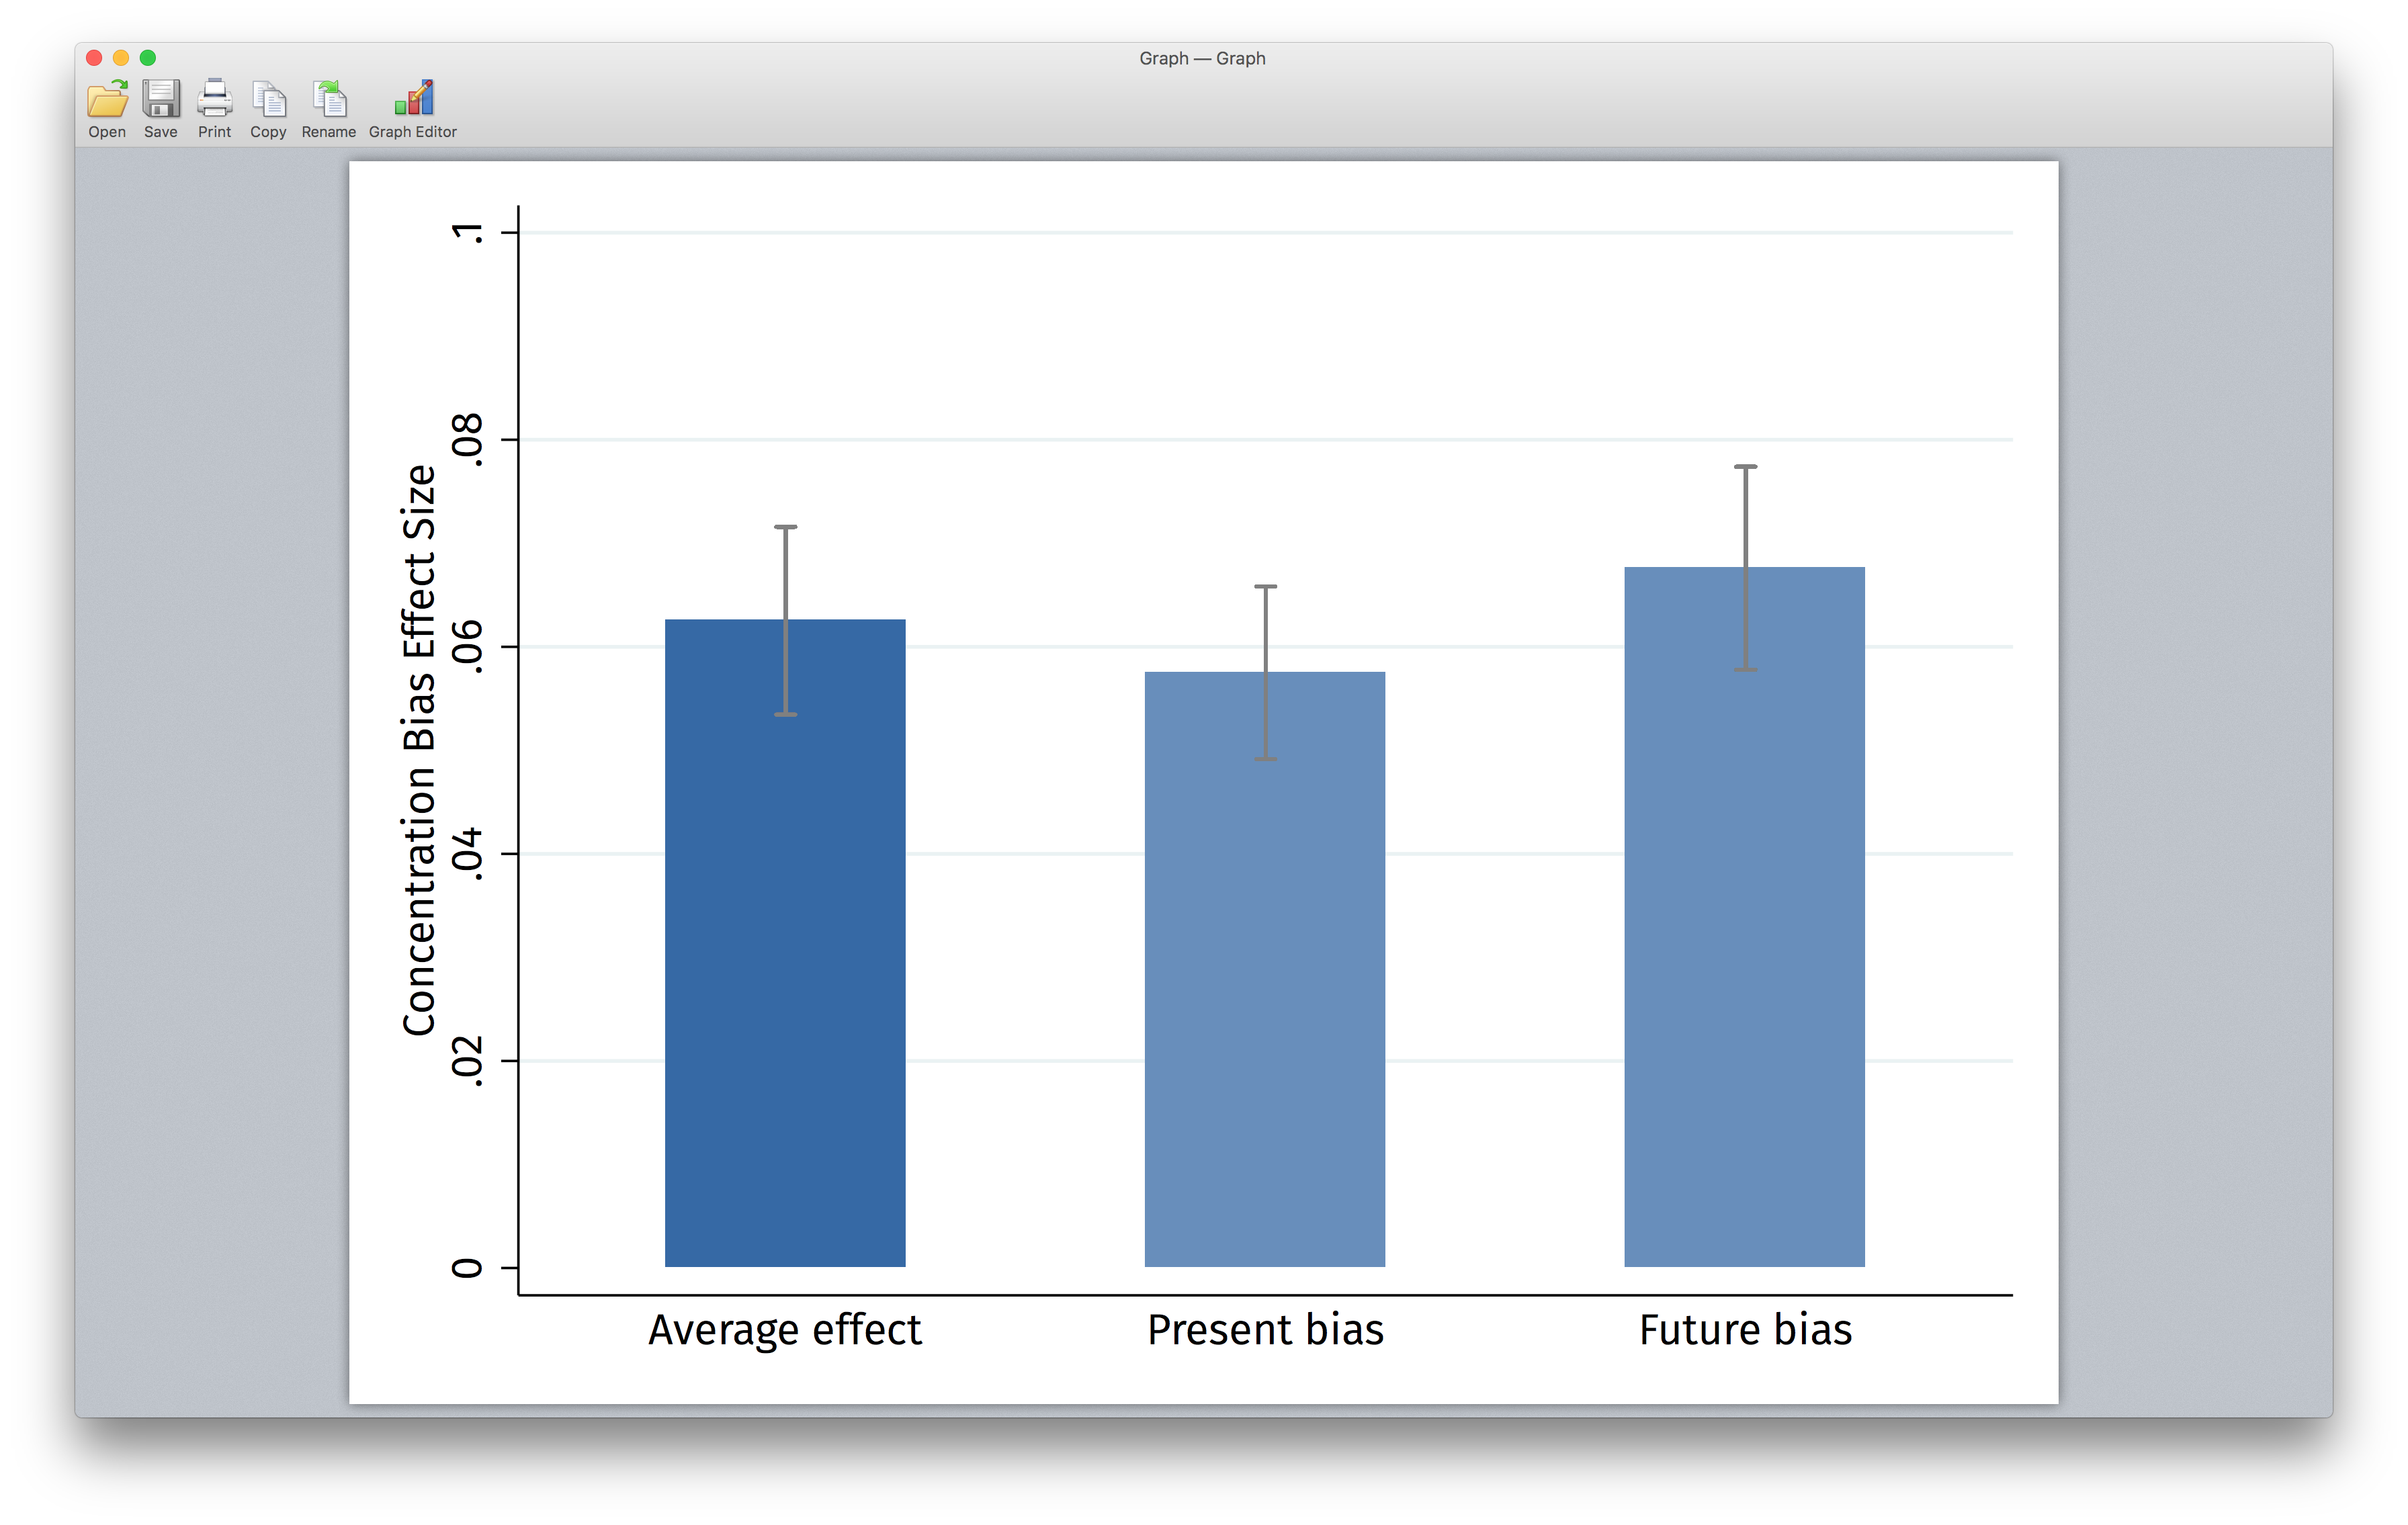
\includegraphics[width=1.643in, trim={3.75in 1.75in 3.75in 2in}, clip]
					{1_Example_Content/Images/average_pb_fb.png} \\
				\centering \footnotesize \sffamily
				$\text{\balA} - \text{\unbalA[\bullet]}$
			\end{minipage}
			\hspace{2pt}
			\begin{minipage}[t]{0.46\textwidth}
				\Large\textbf{B} \textcolor{SpotColor}{\hspace{0.39in} {\small \textbf{Result~2}}} \\[15pt]
				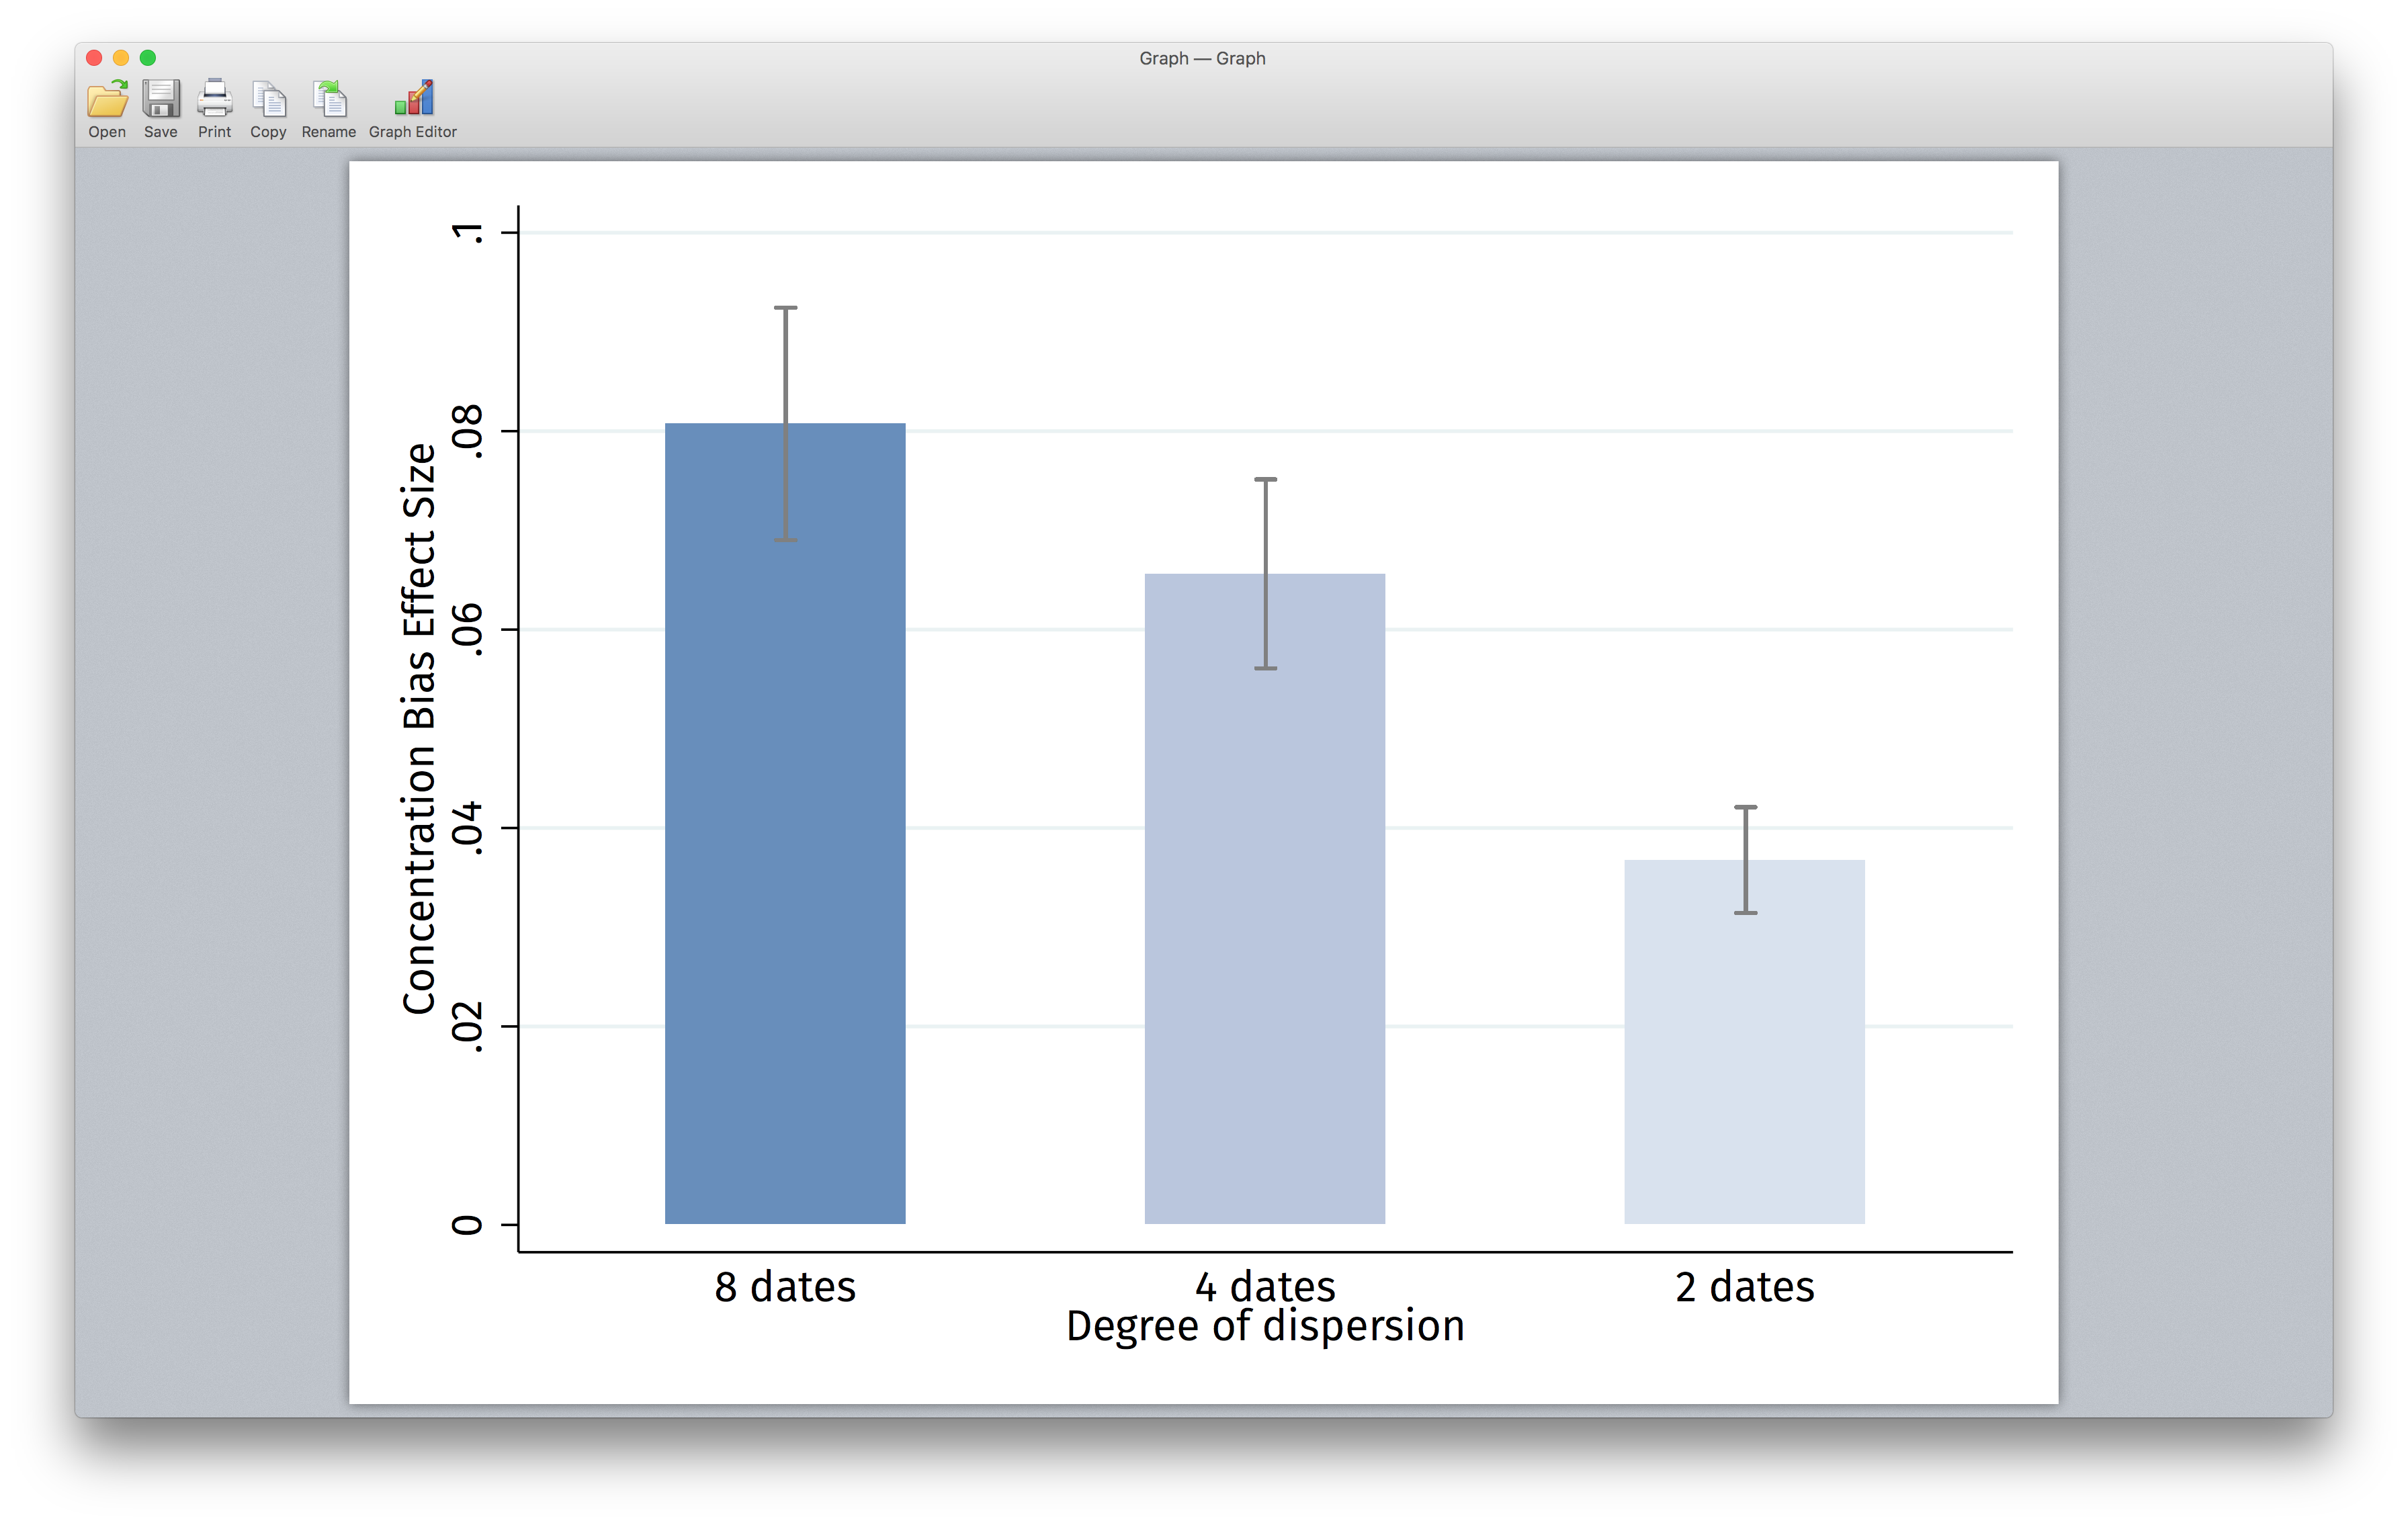
\includegraphics[width=1.710in, trim={3.75in 1.75in 3.75in 2in}, clip]
					{1_Example_Content/Images/average_8_4_2.png} \\
				\centering \footnotesize \sffamily
				$\text{\unbalB[\bullet]} - \text{\balB}$
			\end{minipage} \\
		\end{minipage}
		\caption{%
			\textbf{(A)}~Difference between treatment and control condition. \textbf{(B)}~Heterogeneity.%
		}
	\end{figure}

\end{frame}


\begin{frame}{\titleprefix: Main vs. Control Experiment}

	Rule out some alternative explanations \citep{Dertwinkel-Kalt2017}.

	\bigskip

	\centering
	{\small \alert{Result~3}} \\[15pt]
	% trim={<left> <lower> <right> <upper>}
	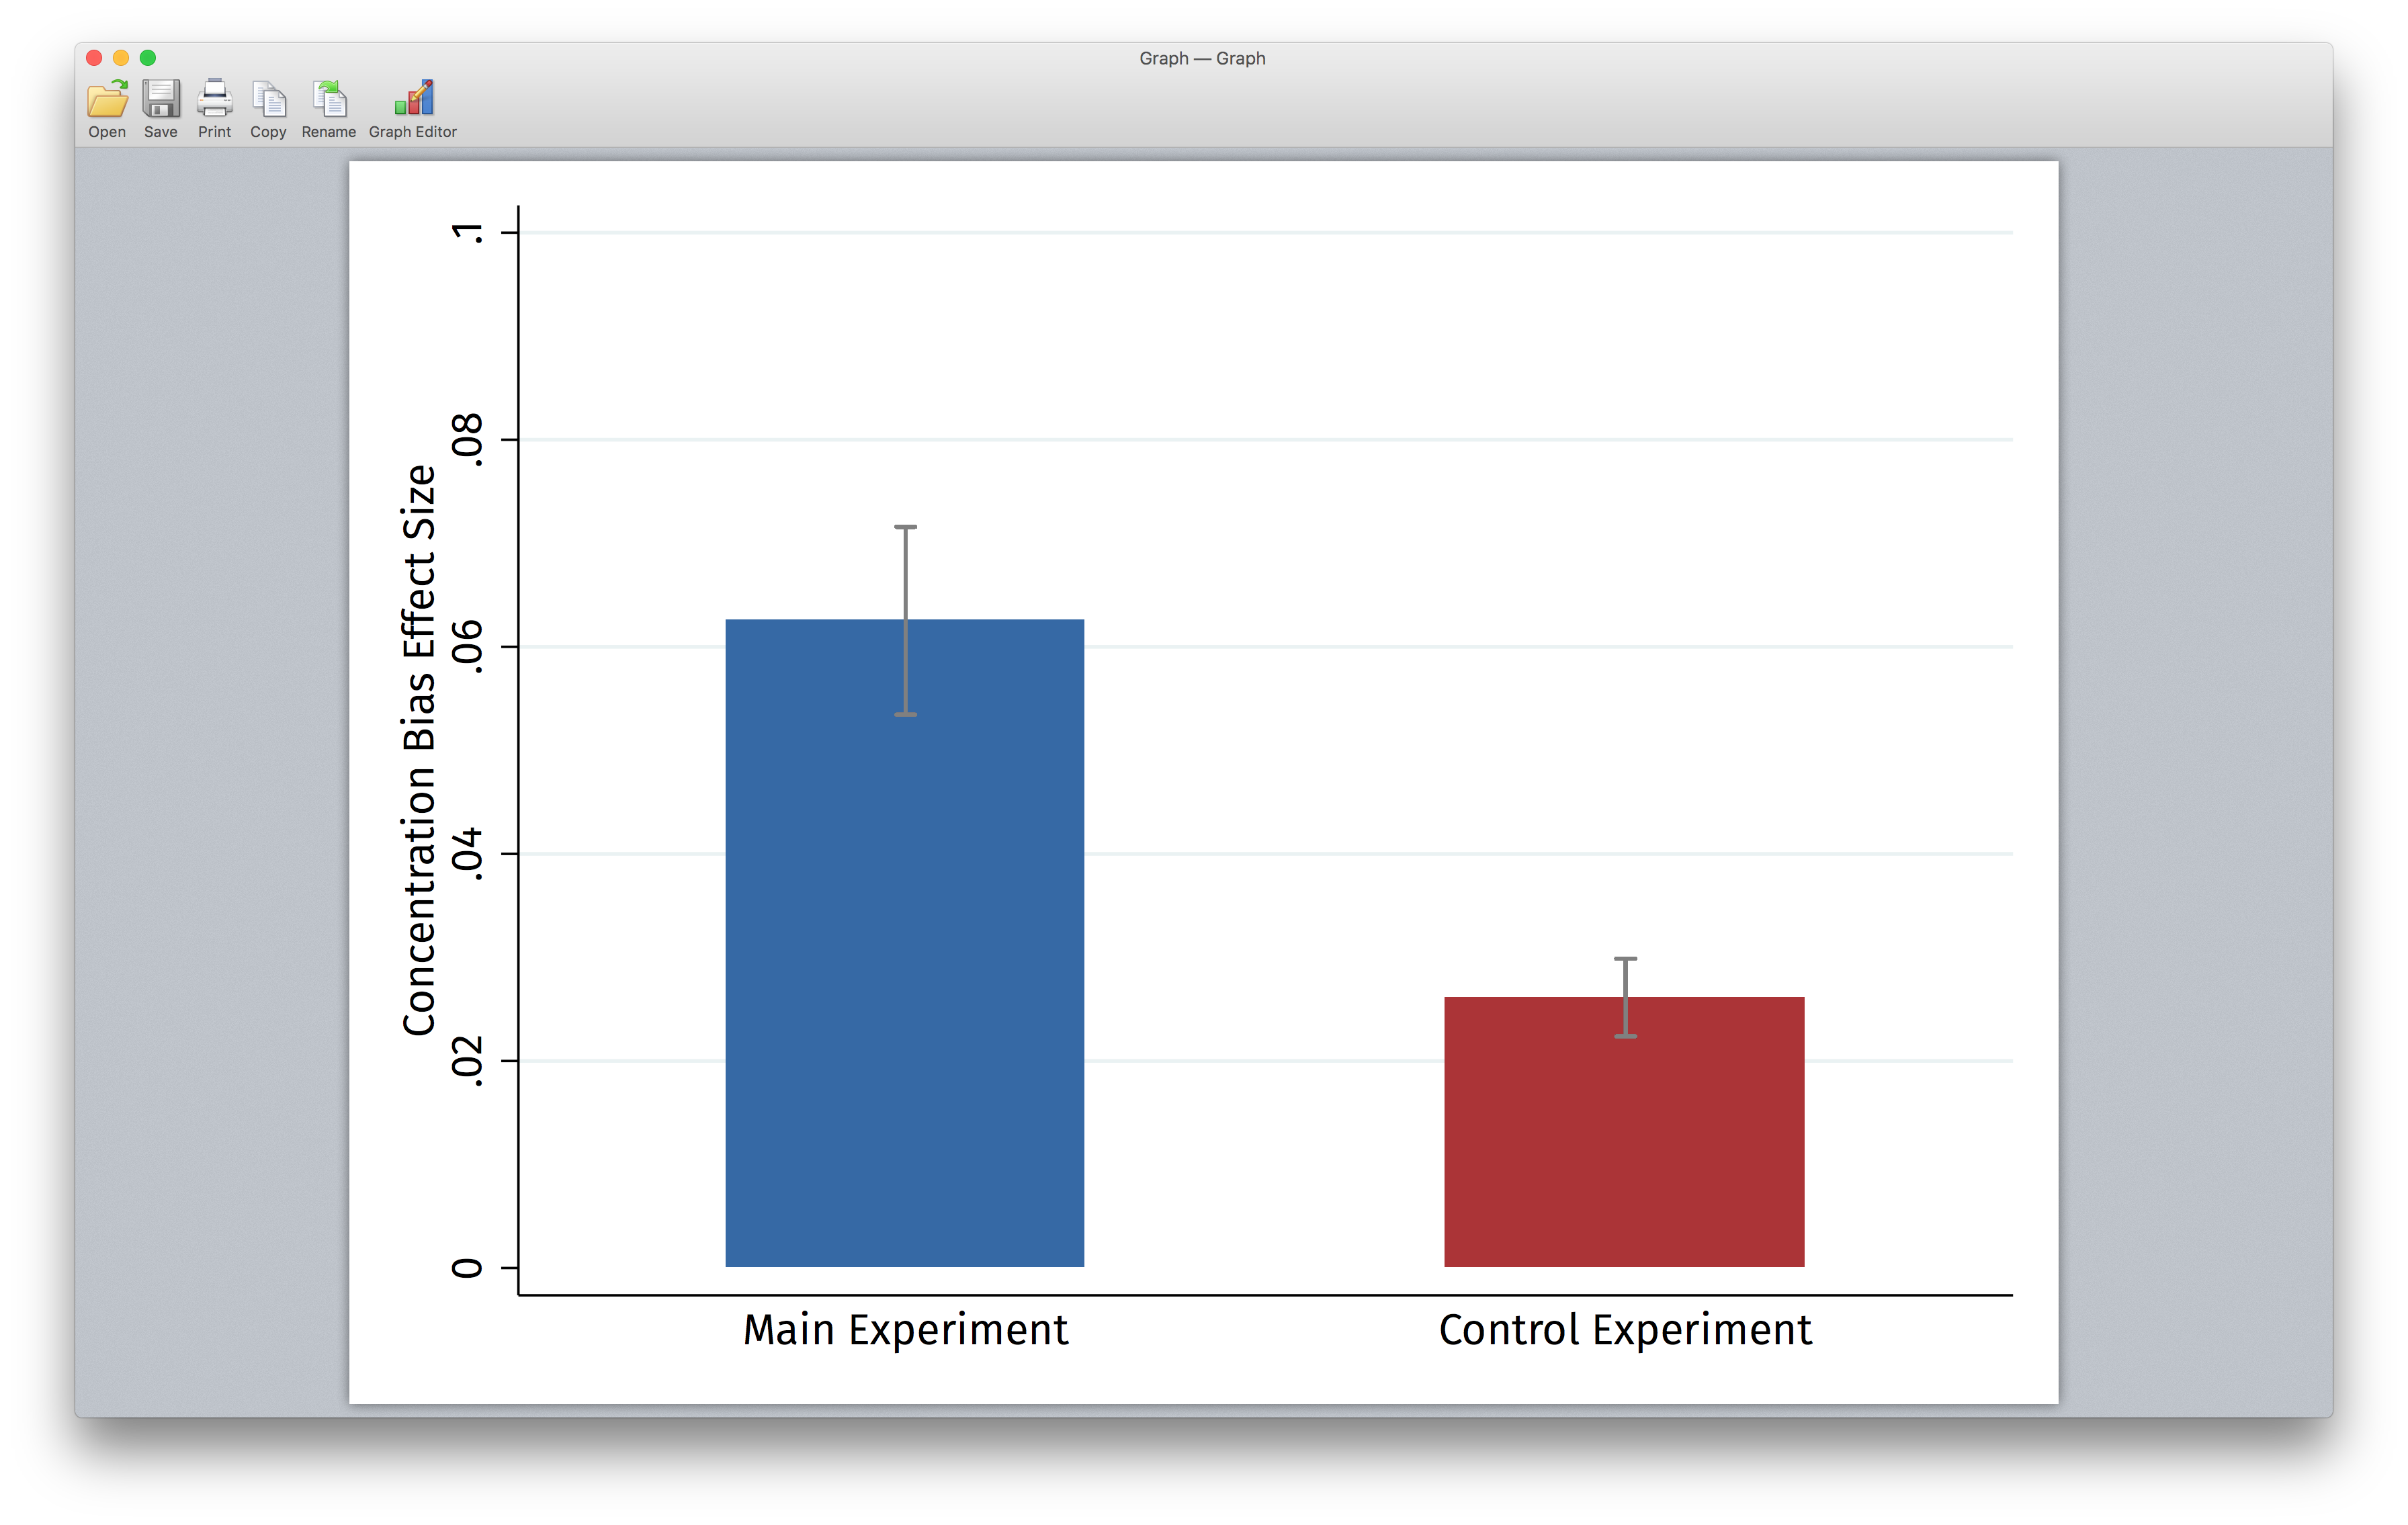
\includegraphics[height=0.5\textheight, trim={3.75in 1.75in 3.75in 2in}, clip]
		{1_Example_Content/Images/average_main_control.png}

\end{frame}


\begin{frame}{\titleprefix: Another \textbf{\texttt{siunitx}} Example Table}

	\begin{table}
	\caption{%
		Example of a~regression table \citep[adapted from][]{Gerhardt2017}.
		Never forget to mention the dependent variable (here, $m_\sim$)!%
	}
	\label{tab:lin_reg_interactions}
	\resizebox*{!}{0.59\textheight}{%
		\mdseries\selectfont
		\footnotesize
\newcolumntype{U}{S[table-format=+1.3, round-mode=places, round-precision=3, table-space-text-pre={**}, table-space-text-post={-**}, round-integer-to-decimal=false]}
\begin{tabularx}
	{\textwidth}
	{@{} L @{\hspace{1.5em}} U @{\hspace{1em}} U @{\hspace{1em}} U @{\hspace{1em}} U @{\hspace{1em}} U @{}}
\toprule
&	{(1)}	&	{(2)}	&	{(3)}	&	{(4)}	&	{(5)} \\
\midrule
Treatment
	&	-0.390	&	-0.228	&	-0.729*	&	-0.449*	&	-0.453**	\\
	&	(+0.352)	&	(-0.205)	&	[+0.377]	&	[-0.245]	&	{\{}+0.204{\}}	\\
Female
	&	0.948***	&	0.0607	&	0.188	&	0.305	&	0.385*	\\
	&	(0.354)	&	(0.233)	&	(0.372)	&	(0.226)	&	(0.222)	\\
$\text{Female} \times \text{Treatment}$
	&	0.169	&	0.251	&	0.892*	&	0.454	&	0.439	\\
	&	(0.514)	&	(0.325)	&	(0.533)	&	(0.341)	&	(0.307)	\\
Final high school grade
	&	-0.101	&	0.0132	&	0.0759	&	0.117	&	0.0394	\\
	&	(0.198)	&	(0.144)	&	(0.224)	&	(0.146)	&	(0.133)	\\
Trait self-control
	&	-0.0156	&	0.00214	&	-0.0160	&	-0.000122	&	-0.00678	\\
	&	(0.0162)	&	(0.00994)	&	(0.0147)	&	(0.0104)	&	(0.00935)	\\
Constant
	&	2.357***	&	1.512***	&	-0.322	&	2.158***	&	1.437***	\\
	&	(0.239)	&	(0.144)	&	(0.265)	&	(0.161)	&	(0.152)	\\
\midrule
Observations
	&	{303}	&	{289}	&	{295}	&	{304}	&	{1191}	\\
$R^2$
	&	0.057	&	0.008	&	0.039	&	0.043	&	0.024	\\
\midrule
$\text{Treatment} \times \text{(1 + Female)}$
	&	-0.221	&	0.0228	&	0.163	&	0.00435	&	-0.0138	\\
$p_F[\text{Treatment} \times {}$ \newline\hspace{12pt}$(1 + \text{Female}) = 0]$
	&	0.327	&	0.00767	&	0.192	&	0.000314	&	0.00343	\\
\bottomrule
\addlinespace
\multicolumn{6}{@{} p{\textwidth} @{}}{%
	\textit{Notes:} Dependent variable: $m_\sim$. Robust standard errors (cluster-corrected for column~5) in parentheses. ***\,${p < 0.01}$, **\,${p < 0.05}$, *\,${p < 0.1}$. Missing observations (${N < 308}$) due to exclusion of trials in which subjects behaved irrationally (i.e., chose a~dominated option). The regressors Final high school grade and Trait self-control are mean-centered.
}
\end{tabularx}
	}
	\end{table}

\end{frame}


\begin{frame}{\titleprefix: Revealing a~Table Column by Column}

	\begin{table}
	\caption{%
		Revealing a~table column-by-column makes it easier to comprehend.%
	}
	\resizebox*{!}{0.59\textheight}{%
		\mdseries\selectfont
		\footnotesize
\newcolumntype{T}{S[table-format=+1.3, round-mode=places, round-precision=3, table-space-text-pre={**}, table-space-text-post={-**}, round-integer-to-decimal=false]}
\begin{tabularx}
	{\textwidth}
	{@{} L<{{\leavevmode\onslide<2->}} @{\hspace{1.5em}} T<{{\leavevmode\onslide<3->}} @{\hspace{1em}} T<{{\leavevmode\onslide<4->}} @{\hspace{1em}} T<{{\leavevmode\onslide<5->}} @{\hspace{1em}} T<{{\leavevmode\onslide<6>}} @{\hspace{1em}} T<{{\leavevmode\onslide}} @{}}
\toprule
&	{(1)}	&	{(2)}	&	{(3)}	&	{(4)}	&	{(5)} \\
\midrule
Treatment
	&	-0.390	&	-0.228	&	-0.729*	&	-0.449*	&	-0.453**	\\
	&	(+0.352)	&	(-0.205)	&	[+0.377]	&	[-0.245]	&	{\{}+0.204{\}}	\\
Female
	&	0.948***	&	0.0607	&	0.188	&	0.305	&	0.385*	\\
	&	(0.354)	&	(0.233)	&	(0.372)	&	(0.226)	&	(0.222)	\\
$\text{Female} \times \text{Treatment}$
	&	0.169	&	0.251	&	0.892*	&	0.454	&	0.439	\\
	&	(0.514)	&	(0.325)	&	(0.533)	&	(0.341)	&	(0.307)	\\
Final high school grade
	&	-0.101	&	0.0132	&	0.0759	&	0.117	&	0.0394	\\
	&	(0.198)	&	(0.144)	&	(0.224)	&	(0.146)	&	(0.133)	\\
Trait self-control
	&	-0.0156	&	0.00214	&	-0.0160	&	-0.000122	&	-0.00678	\\
	&	(0.0162)	&	(0.00994)	&	(0.0147)	&	(0.0104)	&	(0.00935)	\\
Constant
	&	2.357***	&	1.512***	&	-0.322	&	2.158***	&	1.437***	\\
	&	(0.239)	&	(0.144)	&	(0.265)	&	(0.161)	&	(0.152)	\\
\midrule
Observations
	&	{303}	&	{289}	&	{295}	&	{304}	&	{1191}	\\
$R^2$
	&	0.057	&	0.008	&	0.039	&	0.043	&	0.024	\\
\midrule
$\text{Treatment} \times \text{(1 + Female)}$
	&	-0.221	&	0.0228	&	0.163	&	0.00435	&	-0.0138	\\
$p_F[\text{Treatment} \times {}$ \newline\hspace{12pt}$(1 + \text{Female}) = 0]$
	&	0.327	&	0.00767	&	0.192	&	0.000314	&	0.00343	\\
\bottomrule
\end{tabularx}
	}
	\end{table}

\end{frame}


\begin{frame}{\titleprefix: Highlighting Cells in a~Table}

	\begin{table}
	\caption{%
		There are various ways to highlight cells, columns, and rows in a~table.%
	}
	\resizebox*{!}{0.59\textheight}{%
		\mdseries\selectfont
		\newcommand{\highlightrect}[5][2pt]{%
	\makebox(0, 0)[lb]{\hspace{-#2}\raisebox{-#3}[#3][-#3]{%
		\begin{tikzpicture}
			\draw[draw = UBonnYellow, line width = #1] (0, 0) rectangle ++(#4, #5);
		\end{tikzpicture}%
	}}%
}%
% Optional argument: Line width of the frame
% Required argument 1: By how much frame is moved leftwards from current position
% Required argument 2: By how much frame is moved downwards from current position
% Required argument 3: Width of the frame
% Required argument 4: Height
%
% Based on https://tex.stackexchange.com/a/18430/156280:
\def\highlightThisRowOnlyTwo{}%
\only<2>{%
	\def\highlightThisRowOnlyTwo{\rowcolor{UBonnYellow!75}}%
}%
%
\footnotesize
\newcolumntype{T}{S[table-format=+1.3, round-mode=places, round-precision=3, table-space-text-pre={**}, table-space-text-post={-**}, round-integer-to-decimal=false]}
\begin{tabularx}
	{\textwidth}
	{@{} L @{\hspace{1.5em}} T @{\hspace{1em}} T @{\hspace{1em}} >{{{\only<3>{\cellcolor{UBonnYellow!75}}}}}T @{\hspace{1em}} T @{\hspace{1em}} T @{}}
\toprule
&	{(1)}	&	{(2)}	&	{(3)}	&	{\only<5>{\highlightrect[1pt]{2.25em}{35.5ex}{6em}{33.33ex}}(4)}	&	{(5)} \\
\midrule
\highlightThisRowOnlyTwo Treatment
	&	{\only<1>{\cellcolor{UBonnYellow!75}}}-0.390	&	-0.228	&	-0.729*	&	-0.449*	&	-0.453**	\\
	&	(+0.352)	&	(-0.205)	&	[+0.377]	&	[-0.245]	&	{\{}+0.204{\}}	\\
\only<4>{\highlightrect[1pt]{3pt}{3.25pt}{1.01\textwidth}{10.5pt}}Female
	&	0.948***	&	0.0607	&	0.188	&	0.305	&	0.385*	\\
	&	(0.354)	&	(0.233)	&	(0.372)	&	(0.226)	&	(0.222)	\\
$\text{Female} \times \text{Treatment}$
	&	0.169	&	0.251	&	0.892*	&	0.454	&	0.439	\\
	&	(0.514)	&	(0.325)	&	(0.533)	&	(0.341)	&	(0.307)	\\
Final high school grade
	&	-0.101	&	0.0132	&	0.0759	&	0.117	&	0.0394	\\
	&	(0.198)	&	(0.144)	&	(0.224)	&	(0.146)	&	(0.133)	\\
Trait self-control
	&	-0.0156	&	0.00214	&	-0.0160	&	-0.000122	&	-0.00678	\\
	&	(0.0162)	&	(0.00994)	&	(0.0147)	&	(0.0104)	&	(0.00935)	\\
Constant
	&	2.357***	&	1.512***	&	-0.322	&	2.158***	&	1.437***	\\
	&	(0.239)	&	(0.144)	&	(0.265)	&	(0.161)	&	(0.152)	\\
\midrule
Observations
	&	{303}	&	{289}	&	{295}	&	{304}	&	{1191}	\\
$R^2$
	&	0.057	&	0.008	&	0.039	&	0.043	&	0.024	\\
\midrule
$\text{Treatment} \times \text{(1 + Female)}$
	&	-0.221	&	0.0228	&	0.163	&	0.00435	&	-0.0138	\\
$p_F[\text{Treatment} \times {}$ \newline\hspace{12pt}$(1 + \text{Female}) = 0]$
	&	0.327	&	0.00767	&	0.192	&	0.000314	&	0.00343	\\
\bottomrule
\end{tabularx}
	}
	\end{table}

\end{frame}


\begin{frame}{\titleprefix: Yet Another \texttt{siunitx} Example Table}

	\begin{table}
		\caption{Figure grouping via \texttt{siunitx} in a~table.}
		\begin{tabular}
	{ @{}
	  S[table-format=+1.3, table-space-text-pre={**}, table-space-text-post={-**}]
	  S[table-format=+1.5, table-space-text-pre={**}, table-space-text-post={-**}]
	  S[table-format=+6.3, table-space-text-pre={**}, table-space-text-post={-**}]
	  @{}
	}
	\toprule
	{(1)}	&  {(2)}	& {(3)}\\
	\midrule
	-0.100*	& -0.10001*	& -123456.444*** \\
	(2.871) & (2.87123)	& [+50000.123] \\
	\bottomrule
\end{tabular}
	\end{table}

\end{frame}


\section{Discussion}


\begin{frame}{\titleprefix}

	\begin{itemize}[<+->]
		\item The latex exhibits a neutral, acid, or alkaline reaction, depending on the plant from which it was obtained.
		\item The latex is therefore usually allowed to coagulate on the tree \citep{Koszegi2013}.
			\begin{itemize}
				\item<.->[\raisebox{0.75pt}{\scalebox{0.86}{$\Rightarrow$}}\!] The latex, which is usually coagulated by standing or by heating, is obtained from incisions.
			\end{itemize}
		\item See also \cite{Bordalo2013, Dohmen2012}.
	\end{itemize}

\end{frame}


\begin{frame}{\titleprefix: Conclusion}

	A~paragraph before a~list.

	\begin{itemize}
		\item When exposed to air, the latex gradually undergoes putrefactive changes accompanied by coagulation. \par
		A~paragraph within a list item.
		\item The addition of a small quantity of ammonia or of formalin to some latices has the effect of preserving them.
		\item There is, however, reason to believe the following.
		\item The coagulation of latex into rubber is not mainly of this character.
	\end{itemize}

	A~paragraph after a~list.

\end{frame}


\begin{frame}{\titleprefix: An Automated Animation}

The automated transition to the next slide (=~page in the PDF document) only works in full-screen mode.
\begin{itemize}
	\item The feature is available in Adobe Acrobat and Acrobat Reader.
	\item Unfortunately, it is (currently, \today) not available in macOS Preview, Skim, and SumatraPDF.
\end{itemize}
\transduration{0.25}%
\only<12>{\transduration{}}\hypertarget<1>{animation_start}{}%
\foreach \n [evaluate=\n as \angle using \n * 30] in {0, ..., 12}{
	\only<\n>{
		\begin{figure}
			\begin{tikzpicture}
				\draw[draw=none, use as bounding box](-1, 0) rectangle (1, 2);
				\filldraw[fill=SpotColor, draw=none] (0,1) -- (0,2) arc (90:90-\angle:1cm) -- cycle;
			\end{tikzpicture}
			\caption{Step~\n---Angle: \angle\textdegree}
		\end{figure}
	}
}%
\vspace{-\bigskipamount}
\hyperlink<12>{animation_start}{\beamerreturnbutton{Back to the start}}

\end{frame}


\begin{frame}[allowframebreaks]{\titleprefix: Testing the \texttt{allowframebreaks} option}

Let's test automatic numbering with the \texttt{allowframebreaks} option.

On this slide, \textbf{no} number should be included in the frame title.

\end{frame}


\begin{frame}[allowframebreaks]{\titleprefix: Testing the \texttt{allowframebreaks} Option}

\renewcommand{\blindmarkup}[1]{\emph{#1}}

Let's test automatic numbering with the \texttt{allowframebreaks} option.

On this slide, \textbf{``(1/3)''} should appear in the frame title.

\blindtext

\parstart{\framebreak}
\Blindtext[2]

\end{frame}


\section{Math ``Torture'' Test}


\begin{frame}[allowframebreaks]{\insertsection}

\makeatletter
\newcommand*{\checkgreekletters}{%
	\@for\@tempa:=%
	alpha,beta,gamma,delta,epsilon,varepsilon,zeta,eta,theta,vartheta,iota,kappa,lambda,mu,nu,xi,%
	omicron,pi,varpi,rho,varrho,sigma,varsigma,tau,upsilon,phi,varphi,chi,psi,omega,digamma,%
	Alpha,Beta,Gamma,Delta,Epsilon,Zeta,Eta,Theta,Iota,Kappa,Lambda,Mu,Nu,Xi,%
	Omicron,Pi,Rho,Sigma,Tau,Upsilon,Phi,Chi,Psi,Omega,Digamma%
	\do{$\csname\@tempa\endcsname,$ }%
}
\makeatother

\noindent%
{\rmfamily\selectfont\checkgreekletters --- $\mathup{g, \gamma, \Gamma}, \mathbf{g, \gamma, \Gamma}, \mathbfup{g, \gamma, \Gamma}, \mathbfit{g, \gamma, \Gamma}$}

\noindent%
{\rmfamily\selectfont\mathversion{normalup}\upgreekletters\checkgreekletters --- $\mathup{g, \gamma, \Gamma}, \mathbf{g, \gamma, \Gamma}, \mathbfup{g, \gamma, \Gamma}, \mathbfit{g, \gamma, \Gamma}$}

\noindent%
{\rmfamily\bfseries\selectfont\checkgreekletters --- $\mathup{g, \gamma, \Gamma}, \mathbf{g, \gamma, \Gamma}, \mathbfup{g, \gamma, \Gamma}, \mathbfit{g, \gamma, \Gamma}$}

\noindent%
{\rmfamily\bfseries\selectfont\mathversion{boldup}\upgreekletters\checkgreekletters --- $\mathup{g, \gamma, \Gamma}, \mathbf{g, \gamma, \Gamma}, \mathbfup{g, \gamma, \Gamma}, \mathbfit{g, \gamma, \Gamma}$}

\framebreak

\noindent%
{\sffamily\selectfont\checkgreekletters --- $\mathup{g, \gamma, \Gamma}, \mathbf{g, \gamma, \Gamma}, \mathbfup{g, \gamma, \Gamma}, \mathbfit{g, \gamma, \Gamma}$}

\noindent%
{\sffamily\selectfont\mathversion{sansup}\upgreekletters\checkgreekletters --- $\mathup{g, \gamma, \Gamma}, \mathbf{g, \gamma, \Gamma}, \mathbfup{g, \gamma, \Gamma}, \mathbfit{g, \gamma, \Gamma}$}

\noindent%
{\sffamily\bfseries\selectfont\checkgreekletters --- $\mathup{g, \gamma, \Gamma}, \mathbf{g, \gamma, \Gamma}, \mathbfup{g, \gamma, \Gamma}, \mathbfit{g, \gamma, \Gamma}$}

\noindent%
{\sffamily\bfseries\selectfont\mathversion{boldsansup}\upgreekletters\checkgreekletters --- $\mathup{g, \gamma, \Gamma}, \mathbf{g, \gamma, \Gamma}, \mathbfup{g, \gamma, \Gamma}, \mathbfit{g, \gamma, \Gamma}$}

\framebreak

Most of the following examples are taken from \textit{The \TeX book} \citep[][see \url{https://ctan.org/pkg/texbook}]{Knuth1984} and were adapted for \LaTeX\ from Karl Berry's torture test for plain \TeX\ math fonts.

\noindent $x + y - z$, \quad $x + y * z$, \quad $z * y / z$, \quad
$(x+y)(x-y) = x^2 - y^2$,

\noindent $x \times y \cdot z = [x\, y\, z]$, \quad $x\circ y \bullet z$, \quad
$x\cup y \cap z$, \quad $x\sqcup y \sqcap z$, \quad

\noindent $x \vee y \wedge z$, \quad $x\pm y\mp z$, \quad
$x=y/z$, \;\; $x:=y$, \;\; $x\le y \ne z$, \;\; $x \sim y \simeq z$
$x \equiv y \nequiv z$, \;\; $x\subset y \subseteq z$

\noindent $\sin2\theta=2\sin\theta\cos\theta$, \quad
$\hbox{O}(n\log n\log n)$, \quad
$\Pr(X>x)=\exp(-x/\mu)$,

\noindent $\bigl(x\in A(n)\bigm|x\in B(n)\bigr)$, \quad
$\bigcup_n X_n\bigm\|\bigcap_n Y_n$

% page 178

\noindent In-text matrices $\binom{1\,1}{0\,1}$ and $\bigl(\genfrac{}{}{0pt}{}{a}{1}\genfrac{}{}{0pt}{}{b}{m}\genfrac{}{}{0pt}{}{c}{n}\bigr)$.

\framebreak

{
\rmfamily\selectfont
Disambiguation: $0$~O~$O$, $1$~l~I~$|$~$l$~$I$~$/$, $i$~$j$, $rn$~$m$, $\theta$~$\Theta$, $\phi$~$\psi$, --~$-$

Latin vs. Greek: $a$~$\alpha$, $d$~$\delta$, $e$~$\epsilon$, $i$~$\iota$, $k$~$\kappa$, $n$~$\eta$, $o$~$\sigma$, $p$~$\rho$, \textit{\ss} $\beta$, $u$~$\upsilon$, $v$~$\nu$, $w$~$\omega$, $x$~$\chi$, $y$~$\gamma$, $A$~$\Delta$~$\Lambda$, $O$~$\Theta$~$\Omega$, $T$~$\Gamma$, $Y$~$\Upsilon$.
}

Disambiguation: $0$~O~$O$, $1$~l~I~$|$~$l$~$I$~$/$, $i$~$j$, $rn$~$m$, $\theta$~$\Theta$, $\phi$~$\psi$, --~$-$

Latin vs. Greek: $a$~$\alpha$, $d$~$\delta$, $e$~$\epsilon$, $i$~$\iota$, $k$~$\kappa$, $n$~$\eta$, $o$~$\sigma$, $p$~$\rho$, \textit{\ss} $\beta$, $u$~$\upsilon$, $v$~$\nu$, $w$~$\omega$, $x$~$\chi$, $y$~$\gamma$, $A$~$\Delta$~$\Lambda$, $O$~$\Theta$~$\Omega$, $T$~$\Gamma$, $Y$~$\Upsilon$.

\framebreak
% page 142

$$a_0+\frac1{\displaystyle a_1 +
	{\strut \frac1{\displaystyle a_2 +
			{\strut \frac1{\displaystyle a_3 +
					{\strut \frac1{\displaystyle a_4}}}}}}}$$
% page 143
$$\binom{p}{2}x^2y^{p-2} - \frac1{1 - x}\frac{1}{1 - x^2}
=
\frac{a+1}{b}\bigg/\frac{c+1}{d}.$$
%% page 145
$$\sqrt{1+\sqrt{1+\sqrt{1+\sqrt{1+\sqrt{1+x}}}}}$$
$$\sqrt[n]{1+\sqrt[k]{1+\sqrt[5]{1+\sqrt[4]{1+\sqrt[3]{1+x}}}}}$$

\framebreak
%% page 147

$$\left(\frac{\partial^2}{\partial x^2} + \frac{\partial^2}{\partial y^2}\right)
\bigl|\varphi(x+\mathup{i}y)\bigr|^2=0$$

%% page 149

% $$\pi(n)=\sum_{m=2}^n\left\lfloor\biggl(\sum_{k=1}^{m-1}\bigl
% \lfloor(m/k)\big/\lceil m/k\rceil\bigr\rfloor\biggr)^{-1}\right\rfloor.$$

$$\pi(n)=\sum_{m=2}^n\left\lfloor\Biggl(\sum_{k=1}^{m-1}\bigl
\lfloor(m/k)\big/\lceil m/k\rceil\bigr\rfloor\Biggr)^{-1}\right\rfloor.$$

% page 168

$$\int_0^\infty \frac{t - \mathup{i} b}{t^2 + b^2}e^{\mathup{i}at}\,\mathup{d}t=e^{ab}E_1(ab), \quad
a,b > 0.$$

% page 176

$$\mathbf{A} \coloneqq \begin{pmatrix}x-\lambda&1&0\\
0&x-\lambda&1\\
0&0&x-\lambda\end{pmatrix}.$$

\framebreak

$$\left\lgroup\begin{matrix}a&b&c\\ d&e&f\\\end{matrix}\right\rgroup
\left\lgroup\begin{matrix}u&x\cr v&y\cr w&z\end{matrix}\right\rgroup$$
% page 177
$$\mathbf{A} = \begin{pmatrix}a_{11}&a_{12}&\ldots&a_{1n}\\
a_{21}&a_{22}&\ldots&a_{2n}\\
\vdots&\vdots&\ddots&\vdots\\
a_{m1}&a_{m2}&\ldots&a_{mn}\end{pmatrix}$$
$$\mathbf{M}=\bordermatrix{&C&I&C'\cr
	C&1&0&0\cr I&b&1-b&0\cr C'&0&a&1-a}$$

\framebreak
%% page 186

$$\sum_{n=0}^\infty a_nz^n\quad\hbox{converges if}\quad
|z|<\Bigl(\limsup_{n\to\infty}\root n\of{|a_n|}\,\Bigr)^{-1}.$$

$$\frac{f(x+\mathup{\Delta} x)-f(x)}{\mathup{\Delta} x}\to f'(x)
\qquad \hbox{as $\mathup{\Delta} x\to0$.}$$

$$\|u_i\|=1,\qquad u_i\cdot u_j=0\quad\hbox{if $i\ne j$.}$$

%% page 191

$$\hbox{The confluent image of}\quad
\begin{Bmatrix}\hbox{an arc}\hfill\\\hbox{a circle}\hfill\\
\hbox{a fan}\hfill\\\end{Bmatrix}
\quad\hbox{is}\quad
\begin{Bmatrix}\hbox{an arc}\hfill\\
\hbox{an arc or a circle}\hfill\\
\hbox{a fan or an arc}\hfill\end{Bmatrix}.$$

\framebreak
%% page 186

\bgroup
\mathversion{bold}\bfseries
$$\sum_{n=0}^\infty a_nz^n\quad\hbox{converges if}\quad
|z|<\Bigl(\limsup_{n\to\infty}\root n\of{|a_n|}\,\Bigr)^{-1}.$$

$$\frac{f(x+\mathup{\Delta} x)-f(x)}{\mathup{\Delta} x}\to f'(x)
\qquad \hbox{as $\mathup{\Delta} x\to0$.}$$

$$\|u_i\|=1,\qquad u_i\cdot u_j=0\quad\hbox{if $i\ne j$.}$$

%% page 191

$$\hbox{The confluent image of}\quad
\begin{Bmatrix}\hbox{an arc}\hfill\\\hbox{a circle}\hfill\\
\hbox{a fan}\hfill\\\end{Bmatrix}
\quad\hbox{is}\quad
\begin{Bmatrix}\hbox{an arc}\hfill\\
\hbox{an arc or a circle}\hfill\\
\hbox{a fan or an arc}\hfill\end{Bmatrix}.$$
\egroup

\framebreak
%% page 191

\begin{align*}
T(n)\le T(2^{\lceil\lg n\rceil})
&\le c(3^{\lceil\lg n\rceil}-2^{\lceil\lg n\rceil})\\
&<3c\cdot3^{\lg n}\\
&=3c\,n^{\lg3}.
\end{align*}
%\begin{align*}
%\left\{%
%\begin{gathered}\alpha&=f(z)\\ \beta&=f(z^2)\\ \gamma&=f(z^3)
%\end{gathered}
%\right\}
%\qquad
%\left\{%
%\begin{gathered}
%x&=\alpha^2-\beta\\ y&=2\gamma
%\end{gathered}
%\right\}%
%\end{align*}
%$$\left\{
%\begin{align}
%\alpha&=f(z)\cr \beta&=f(z^2)\cr \gamma&=f(z^3)\\
%%\end{align}
%\right\}
%\qquad
%\left\{
%%\begin{align}
%x&=\alpha^2-\beta\cr y&=2\gamma\\
%\end{align}
%\right\}.$$
%%% page 192
\begin{align*}
\begin{aligned}
(x+y)(x-y)&=x^2-xy+yx-y^2\\
&=x^2-y^2\\
(x+y)^2&=x^2+2xy+y^2.
\end{aligned}
\end{align*}

\framebreak
%% page 192

\begin{align*}
\begin{aligned}
\left( \int\limits_{-\infty}^\infty \mathup{e}^{-x^2}\,\mathup{d}x \right)^2
&=\int_{-\infty}^\infty\int_{-\infty}^\infty \mathup{e}^{-(x^2+y^2)}\,\mathup{d}x\,\mathup{d}y\\
&=\int_0^{2\piup}\int_0^\infty \mathup{e}^{-r^2}\,\mathup{d}r\,\mathup{d}\theta\\
&=\int_0^{2\piup}\biggl(\mathup{e}^{-\frac{r^2}{2}}
\biggl|_{r=0}^{r=\infty}\,\biggr)\,\mathup{d}\theta\\
&=\piup.
\end{aligned}
\end{align*}

\framebreak
%% page 197

$$\prod_{k\ge0}\frac{1}{(1-q^kz)}=
\sum_{n\ge0}z^n\bigg/\!\!\prod_{1\le k\le n}(1-q^k).$$

$$\sum_{\substack{\scriptstyle 0< i\le m\\\scriptstyle0<j\le n}}p(i,j) \,\ne
%
% $$\sum_{i=1}^p \sum_{j=1}^q \sum_{k=1}^r a_{ij} b_{jk} c_{ki}$$
%
\sum_{i=1}^p \sum_{j=1}^q \sum_{k=1}^r a_{ij} b_{jk} c_{ki} \,\ne
%
\sum_{\substack{\scriptstyle 1\le i\le p \\ \scriptstyle 1\le j\le q\\
		\scriptstyle 1\le k\le r}} a_{ij} b_{jk} c_{ki}$$

\framebreak

$$\max_{1\le n\le m}\log_2P_n \quad \hbox{and} \quad
\lim_{x\to0}\frac{\sin x}{x}=1$$
Inline math:
$\max_{1\le n\le m}\log_2P_n \quad \hbox{and} \quad
\lim_{x\to0}\frac{\sin x}{x}=1$
$$p_1(n)=\lim_{m\to\infty}\sum_{\nu=0}^\infty\bigl(1-\cos^{2m}(\nu!^n\piup/n)\bigr)$$
Inline math:
$p_1(n)=\lim_{m\to\infty}\sum_{\nu=0}^\infty\bigl(1-\cos^{2m}(\nu!^n\piup/n)\bigr)$

\end{frame}




%%%%%%%%%%%%%%%%%%
%%  REFERENCES  %%
%%%%%%%%%%%%%%%%%%


\section{\refname}
%\renewcommand\bibsection{}
%	% To prevent ``References'' from appearing twice in the navigation bar

\begin{frame}[allowframebreaks]{\insertsection}

	\begin{refcontext}[sorting=nyt]
		% Sort BIBLIOGRAPHY by alphabet (while CITATIONS are sorted by year)
	\printbibliography[heading=none]
	\end{refcontext}

	%% Only when using BibTeX instead of BibLaTeX ==>
	%\bibliographystyle{0_0_Preamble/aea_doi_url_href}
	%\bibliography{Library}
	%% <==

\end{frame}




%%%%%%%%%%%%%%%%
%%  APPENDIX  %%
%%%%%%%%%%%%%%%%


\begin{appendix}


\section[Appendix\newline \textmd{Backup Slides}]{Appendix}


\begin{frame}[label=model]

	\frametitle{\insertsection: Modeling Concentration Bias}

	Subjects consider a sequences of consequences $\boldsymbol{c}$ from choice set $\boldsymbol{C}$.

	%Focusing theory augments discounted utility (constant, hyperbolic, \dots) through an~additional weight \highlight{$g[\cdot]$} on the instantaneous utility function.
	\begin{itemize}

	\item \alert{Standard discounted utility:}
		Suppose that the instantaneous utility function $u$ satisfies ${u'>0}$ and ${u''\leq 0}$, and that earlier consequences are preferred over later consequences of the same magnitude, i.e., ${D(t)\leq 1}$:
	\item[] ${U}(\boldsymbol{c}\phantom{, \boldsymbol{C}}) \coloneqq
		\sum_{t=1}^{T} \phantom{g_t} D(t)\,u(c_t)$, \quad where, e.g., \quad $D(t) = \delta^t$  or $D(t) = \frac{1}{1 + k\,t}$. %$\beta \delta^t$.
	\medskip
	\item \only<1->{\alert{Focusing model \citep{Koszegi2013}:}}
	\item[]<1-> $\tilde{U}(\boldsymbol{c}\highlight{, C}) \coloneqq \sum_{t=1}^{T} \highlight{g_t}\,D(t)\,u(c_t)$, \quad where \\[3pt]
		\highlight{$g_t \equiv % g[\Delta_t(C)]$, $\Delta_t(C) =
		g[\max_{\boldsymbol{c}'\in C} D(t)\,u(c'_t) - \min_{\boldsymbol{c}'\in C} D(t)\,u(c'_t)]$}
		\smallskip
		\begin{itemize}
			\item<1-> Weighting function \highlight{$g[\cdot]$} increases in difference of maximum and minimum possible utility at a~point in time.
			\item<1-> Subjects overweight intertemporal consequences with a greater range.
		\end{itemize}
	\end{itemize}

\end{frame}


\end{appendix}

\end{document}